\documentclass{beamer}

% Tema de la presentación
\usetheme{Berlin} % Puedes cambiarlo a: Warsaw, Berlin, AnnArbor, etc.
\usepackage{graphicx}
\usepackage{multicol}




% Información del título
\title[Creación de un dashboard para usuarios del ticket digital de Mercadona]{Creación de un dashboard para usuarios del ticket digital de Mercadona con visualización gráfica de datos: evolución de precios por producto, gastos por categoría de alimentación y ventanas temporales de gastos}
\author{Santiago Sánchez Sans}
\institute{IES Abastos}
\date{6 junio 2025} % o una fecha específica


\setbeamertemplate{footline}[frame number]

\begin{document}



	% Portada
	\begin{frame}
		\titlepage
	\end{frame}
	
	% Índice UNA COLUMNA
	\begin{frame}
		\frametitle{Contenido}
		\tableofcontents
	\end{frame}
	
	% Índice DOS COLUMNAS
	%\begin{frame}
	%	\frametitle{Contenido}
	%	\begin{multicols}{2}
		%		\tableofcontents
		%	\end{multicols}
	%\end{frame}

	
	
	% INDICE CON DIFUMINADOS A CADA SECCION
	\AtBeginSection[]{
		\begin{frame}
			\frametitle{Contenidos}
			\tableofcontents[currentsection]
		\end{frame}
	}
	
	% INDICE CON DIFUMINADOS A CADA SECCION (2 COLS)
	%\AtBeginSection[]{
		%	\begin{frame}
			%		\frametitle{Contenidos}
			%		\begin{multicols}{2}
				%			\tableofcontents[currentsection]
				%		\end{multicols}
			%	\end{frame}
		%}

	
	
	
	
	
	% Sección 1: Introducción
	\section{Introducción}
	

\begin{frame}
	\frametitle{1. Introducción}
	\begin{itemize}
		\item \textbf{Identificación de necesidades}:
		\begin{itemize}
			\item Usuario del ticket digital $\rightarrow$ no tiene informes de sus datos.
		\end{itemize}
		
		\item \textbf{Objetivos}:
		\begin{itemize}
			\item Proporcionar al usuario del ticket digital una herramienta que muestre en gráficos visuales:
			\begin{itemize}
				\item \textbf{Evolución de precios} (inflación) a lo largo del tiempo en los productos habitualmente obtenidos en el mismo establecimiento\footnote{La evolución de precios se mostrará solamente para un mismo centro de Mercadona, dado que distintos centros pueden cambiar los nombres de los productos (por ejemplo, en Cataluña…)}.
				\item \textbf{Evolución del gasto} total del usuario a lo largo del tiempo por períodos temporales.
			\end{itemize}
		\end{itemize}
	\end{itemize}
\end{frame}

			
			
			

			
			

	
	
	
	
	
		% Sección 2
		\section{Diseño}
	
	


			
			\subsection{Requisitos}
				% DIAPO REQUISITS
				\begin{frame}
					\frametitle{Requisitos de los usuarios}
					
					Que los usuarios tengan una cuenta de gmail con tickets digitales de Mercadona dentro e, idealmente, tenga decenas de tickets digitales: idealmente con compras estables y productos de adquisición recurrentes.
		
				\end{frame}
				
		
			
	
			
			
		
				% DIAPO REQUISITS funcionals
				\begin{frame}
					\frametitle{Requisitos funcionales}
					
					
					\textbf{REQUISITO A:} Mostrar\textbf{ \textit{evolución de los precios}} de los productos unitarios adquiridos \underline{con más frecuencia} (visualizable en un gráfico donde en X tendremos el tiempo y en Y el precio en euros).
					
					\textbf{REQUISITO B:} Mostrar {\textbf{gasto total en distintas ventanas temporales}} del usuario: períodos de 1, 3, 6 meses y un año; independientemente del centro de Mercadona en el que se compre (todos juntos).
					
					\textbf{REQUISITO C:} Al lado del gasto total anterior se incluirá un \textbf{\textit{diagrama de sectores}} desglosando \underline{porcentaje de dinero} gastado en 13 categorias \href{https://shorturl.at/whzPf}{\color{blue}{(click para ver categorías)}}
					
				\end{frame}
				
				
				
							
				% DIAPO REQUISITS funcionals continuaco
				\begin{frame}
					\frametitle{Requisitos funcionales (cont.)}
					
				
					
					%REQUISIT D I E NO EREN A LA REDACCCIO DEL PROJECTE INICIAL CREC
					\textbf{REQUISITO D\footnote{Requisito añadido después de la presentación inicial del proyecto.}:} Los PDFs descargados del correo del usuario se almacenarán en una carpeta local del ordenador del usuario.
					
					\textbf{REQUISITO E\footnote{Requisito añadido después de la presentación del proyecto.}:} El sistema front-end y back-end de registro permitirá redirigir a los usuarios rápidamente a un registro de forma inteligente. Nos inspiraremos en el sistema de  registro e iniciar sesión de NetFlix. Ver diagrama enrutamiento.
	
				\end{frame}
			
			
			
									
						% DIAPO REQUISITS funcionals RESUM
				\begin{frame}
					\frametitle{Requisitos funcionales (RESUMEN)}
					
					
					De los requisitos al diseño (anticipo de lo que será el dashboard):
				
					\begin{itemize}
						\item evolución de precios por producto $\rightarrow$ \textbf{``inflalyzer''}
						\item gastos por categoría de alimentación $\rightarrow$  \textbf{``categoryzer''}
						\item ventanas temporales de gastos $\rightarrow$  \textbf{``intervalizer''}
					\end{itemize}
					
				\end{frame}
			
			
			
			
			
		
		
		
		
		
		
		
		
		\subsection{Diagramas de sistemas}
		
			% DIAPO DIAGRAMA DE SISTEMES GENERAL
			\begin{frame}
				\frametitle{Diagrama general}
				
				
				\begin{figure}
					\centering
					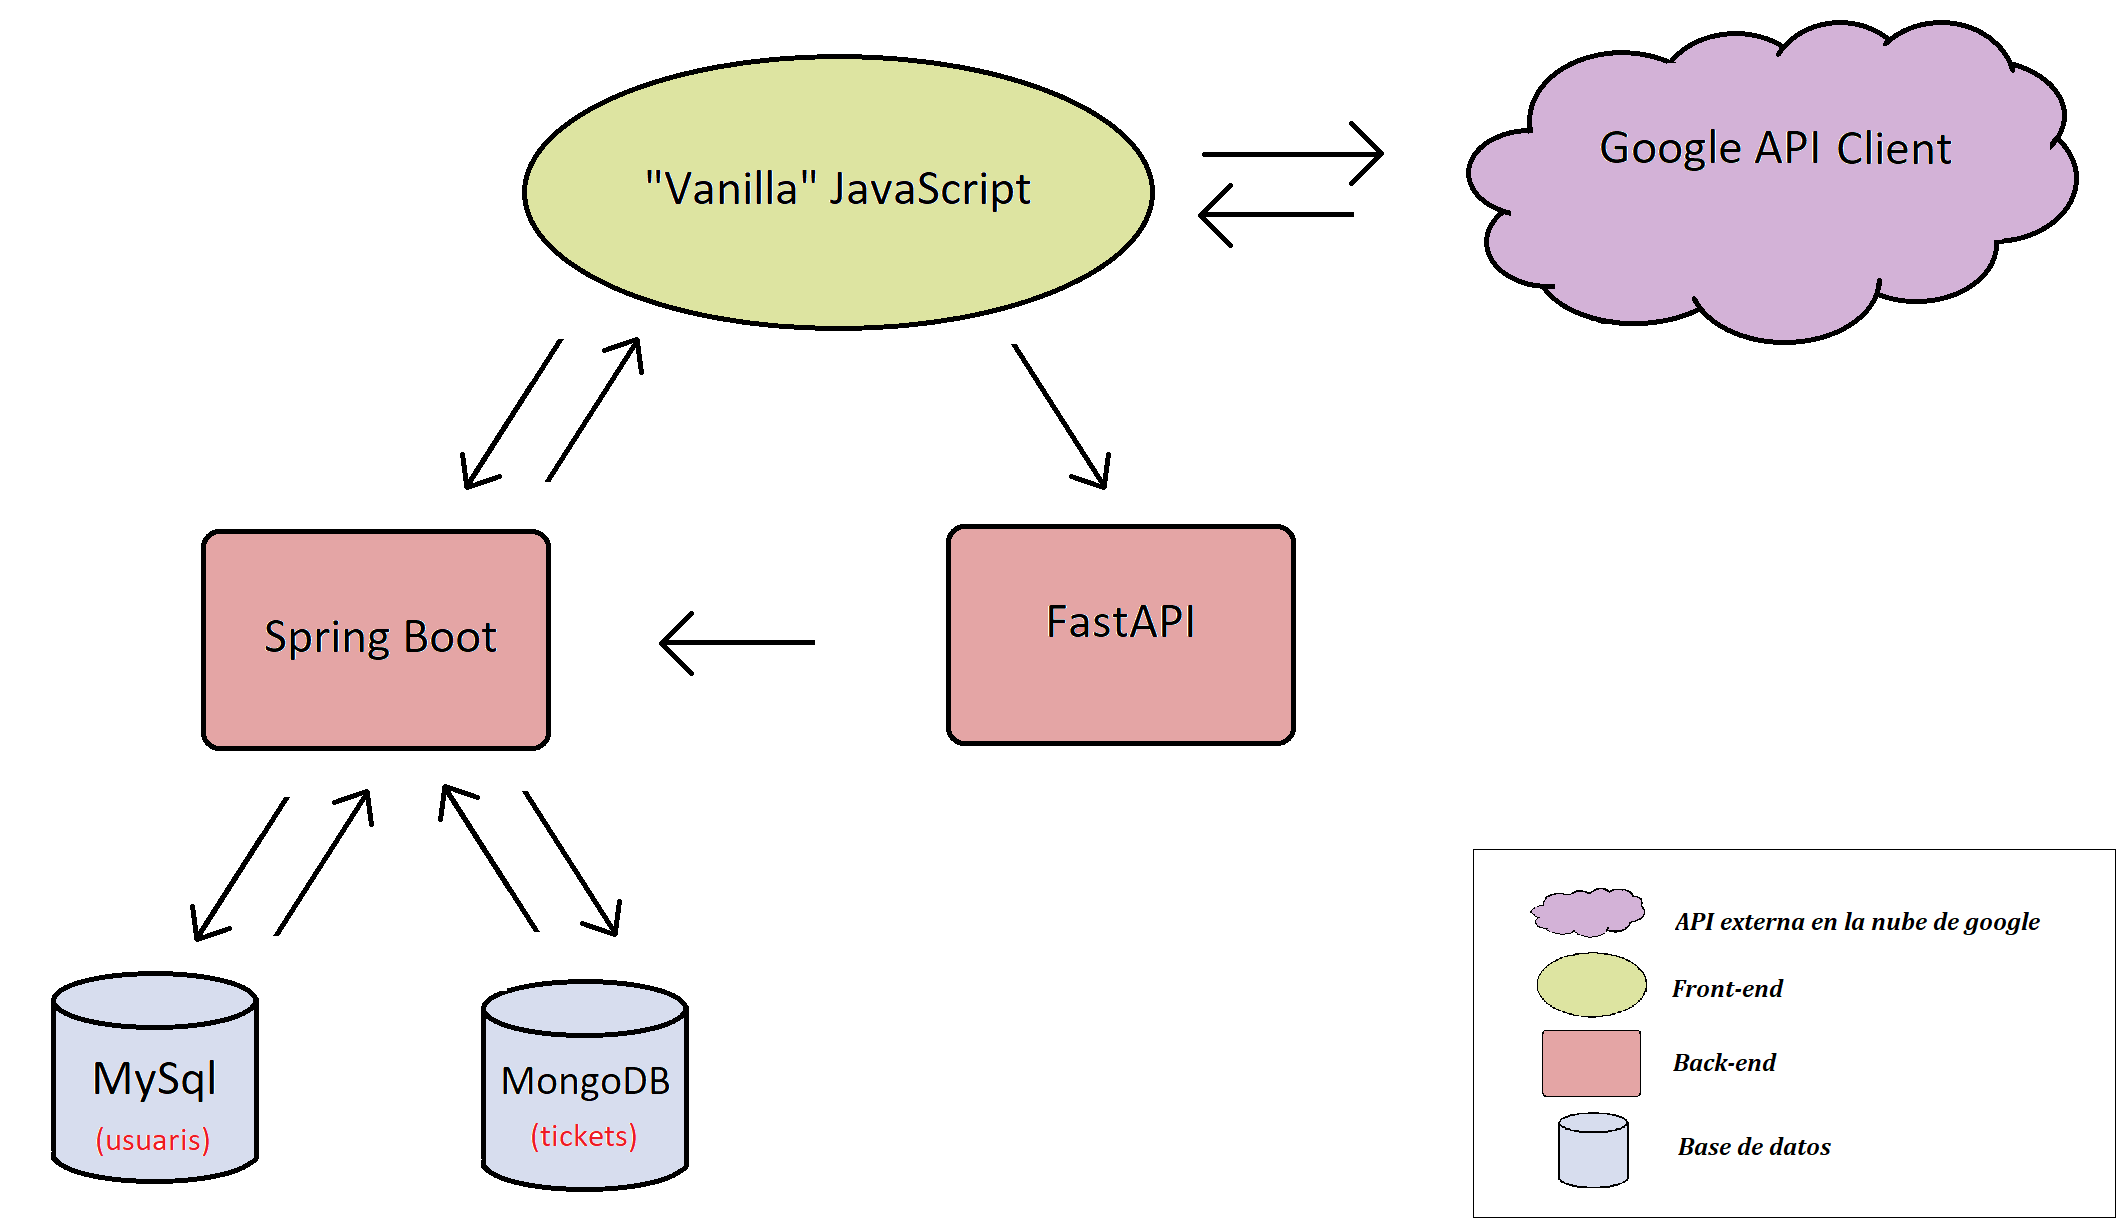
\includegraphics[width=1\linewidth]{../img/diagramaSistemesAplicacioMercapp}
					
					\label{fig:diagramasistemesaplicaciomercapp}
				\end{figure}
				
			\end{frame}
			
			
			% DIAPO DIAGRAMA SISTEMES: REGISTRE (SIMPLIFICAT)
			\begin{frame}
				\frametitle{registro}
				
				\begin{figure}
					\centering
					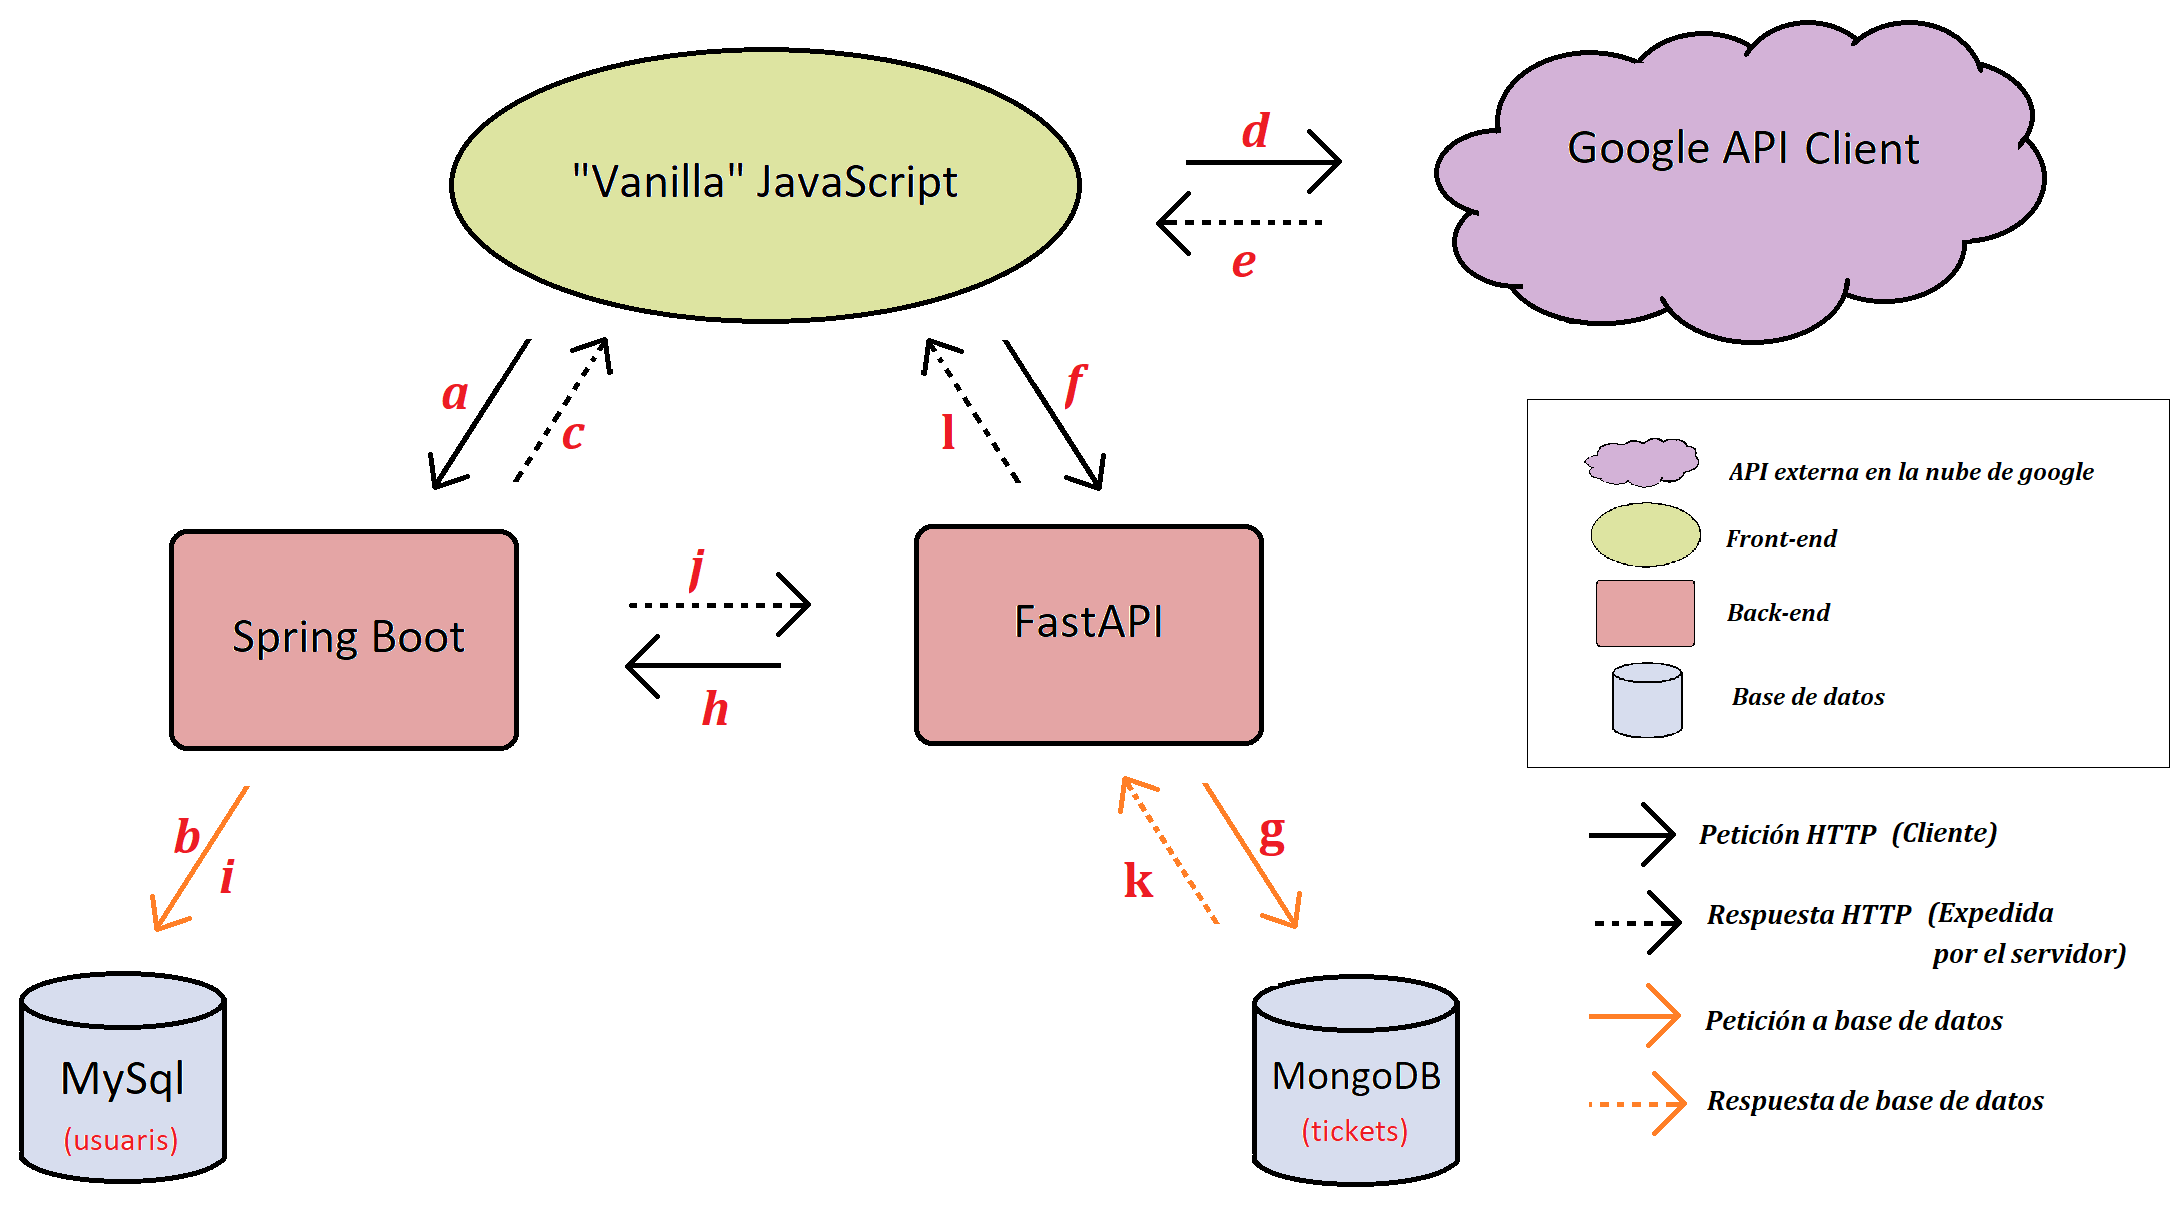
\includegraphics[width=1\linewidth]{../img/diagramaSistemesAplicacioMercappCAMIREGISTREbo}
					
					\label{fig:diagramasistemesaplicaciomercappcamiregistrebo}
				\end{figure}
				
			\end{frame}
			
			
			% DIAPO DIAGRAMA SISTEMES: REGISTRE (INICI SESSIÓ)
			\begin{frame}
				\frametitle{inicio de sesión}
				
				\begin{figure}
					\centering
					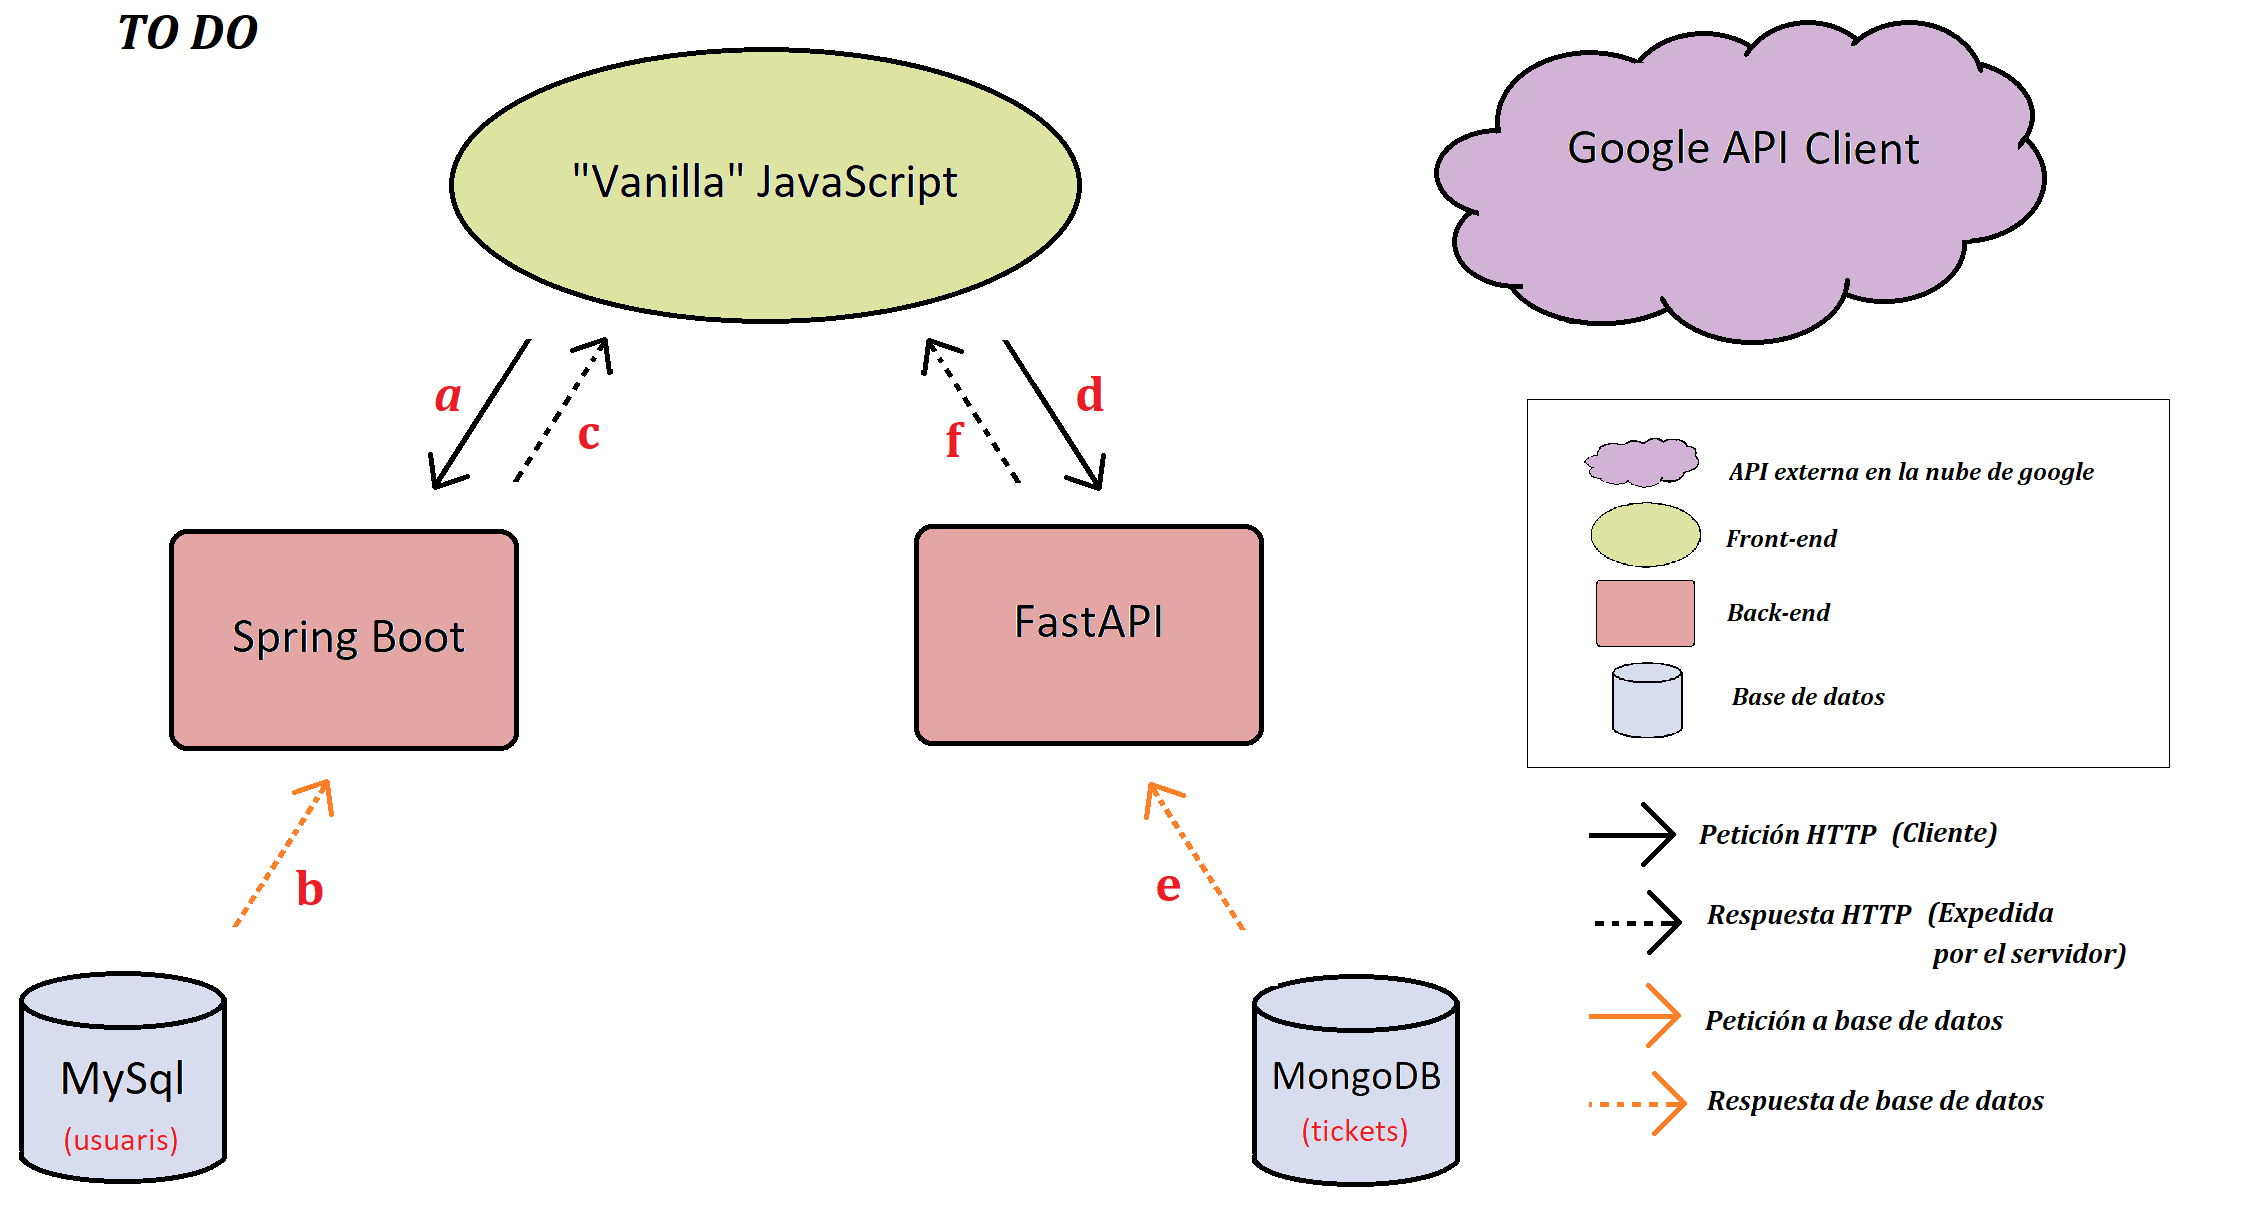
\includegraphics[width=1\linewidth]{../img/diagramaSistemesAplicacioMercappCAMIINICISESSIO}
					
					\label{fig:diagramasistemesaplicaciomercappcamiinicisessio}
				\end{figure}
				
			\end{frame}
			
		
		
		
		
	% Sección 3
	\section{Desarrollo}
	
	
	
	
	% FER AQUI LA DIAPO INICIAL PER MOSTRAR LES PARTS DE DESARROLLO
	
		
	%LA DIAPO QUE EXPLICA EL QUE HI HAAL DISENY

	
	
	
	\subsection{Entornos de desarrollo}
	\begin{frame}
		\frametitle{Entornos de desarrollo}
					
		\begin{table}[h!]
			\centering
			\begin{tabular}{|l|l|}
				\hline
				\textbf{Editor / Herramienta} & \textbf{Puerto\footnote{El host es localhost})} \\
				\hline
				IntelliJ IDEA (Java, SpringBoot) & 8080 \\
				VSCode (HTML, CSS, JS con Live Server) & 5500 \\
				VSCode (Python, con FastAPI\footnote{No depende del editor de código}) & 8000 \\
				MySQL Workbench & 3306 \\
				MongoDB Compass & 27017 \\
				\hline
			\end{tabular}
			\caption{Entornos de desarrollo y puertos utilizados para despliegue en local}
		\end{table}
	\end{frame}
	
	
	
	

	\subsection{Despliegue}
	\begin{frame}
		\frametitle{Despliegue}
		Se ha automatizado la creación de imágenes e instanciado de contenedores para cada microservicio. PUERTOS: ¡idem!
		
		\begin{figure}
			\centering
			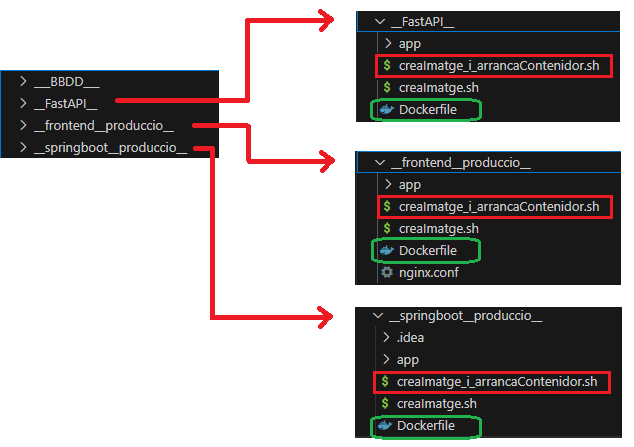
\includegraphics[width=.7\linewidth]{../img/dockeritzacioAplicacioPlantilla}
			\label{fig:dockeritzacioaplicacioplantilla}
		\end{figure}
	\end{frame}
	
	
	\begin{frame}
		\frametitle{Despliegue (cont.)}
		
		
		\begin{table}[h!]
			\centering
			\begin{tabular}{|l|l|}
				\hline
				\textbf{Imagen original} & \textbf{puerto} \\
				\hline
				
				openjdk:17-alpine & 8080 \\
				nginx:alpine & 5500\footnote{localhost no sirve; usar 127.0.0.1 en navegador para ver index.html} \\
				Python:alpine (\href{https://shorturl.at/YdNuy}{\color{blue}{DF}}) & 8000 \\
		
				\hline
			\end{tabular}
			\caption{Imágenes docker base y puertos donde instanciamos su contenedor}
		\end{table}		
	
	
		\begin{table}[h!]
		\centering
			\begin{tabular}{|l|l|}
				\hline
				\textbf{base de datos} & \textbf{puerto} \\
				\hline
				
				\color{red}{MySQL} & 3306 \\
				\color{red}{MongoDB} & 27017 \\
		
				\hline
			\end{tabular}
			\caption{Bases de datos: no contenerizadas}
		\end{table}		
	\end{frame}
	
	
	
	
	\begin{frame}
		\frametitle{CONTINUAR PER 3.4 DE LA MEMORIA EN APARTAT DESARROLLO}
		\textbf{ometre dockeritzacio que surti a desarrollo de la memoria perque ja s'ha posat lo basic a disseny per no repetir.}
		\textbf{Posar sobretot estructures projectes i NO oblidar el diagrama d'enrutament.}
	\end{frame}
	
	
	
	
	\subsection{Spring Boot: gestión usuarios}
	
	
	
	\begin{frame}
		\frametitle{Spring boot aqui}
	\end{frame}
	
	
	%continuar spring boot aqui
	
	
	
	
	
	
	
	\subsection{FastAPI: parseo de tickets}
	
	


		\begin{frame}
		\frametitle{Posar fastapi aqui}
		
		
		\end{frame}


		\begin{frame}
			\begin{figure}
				\centering
				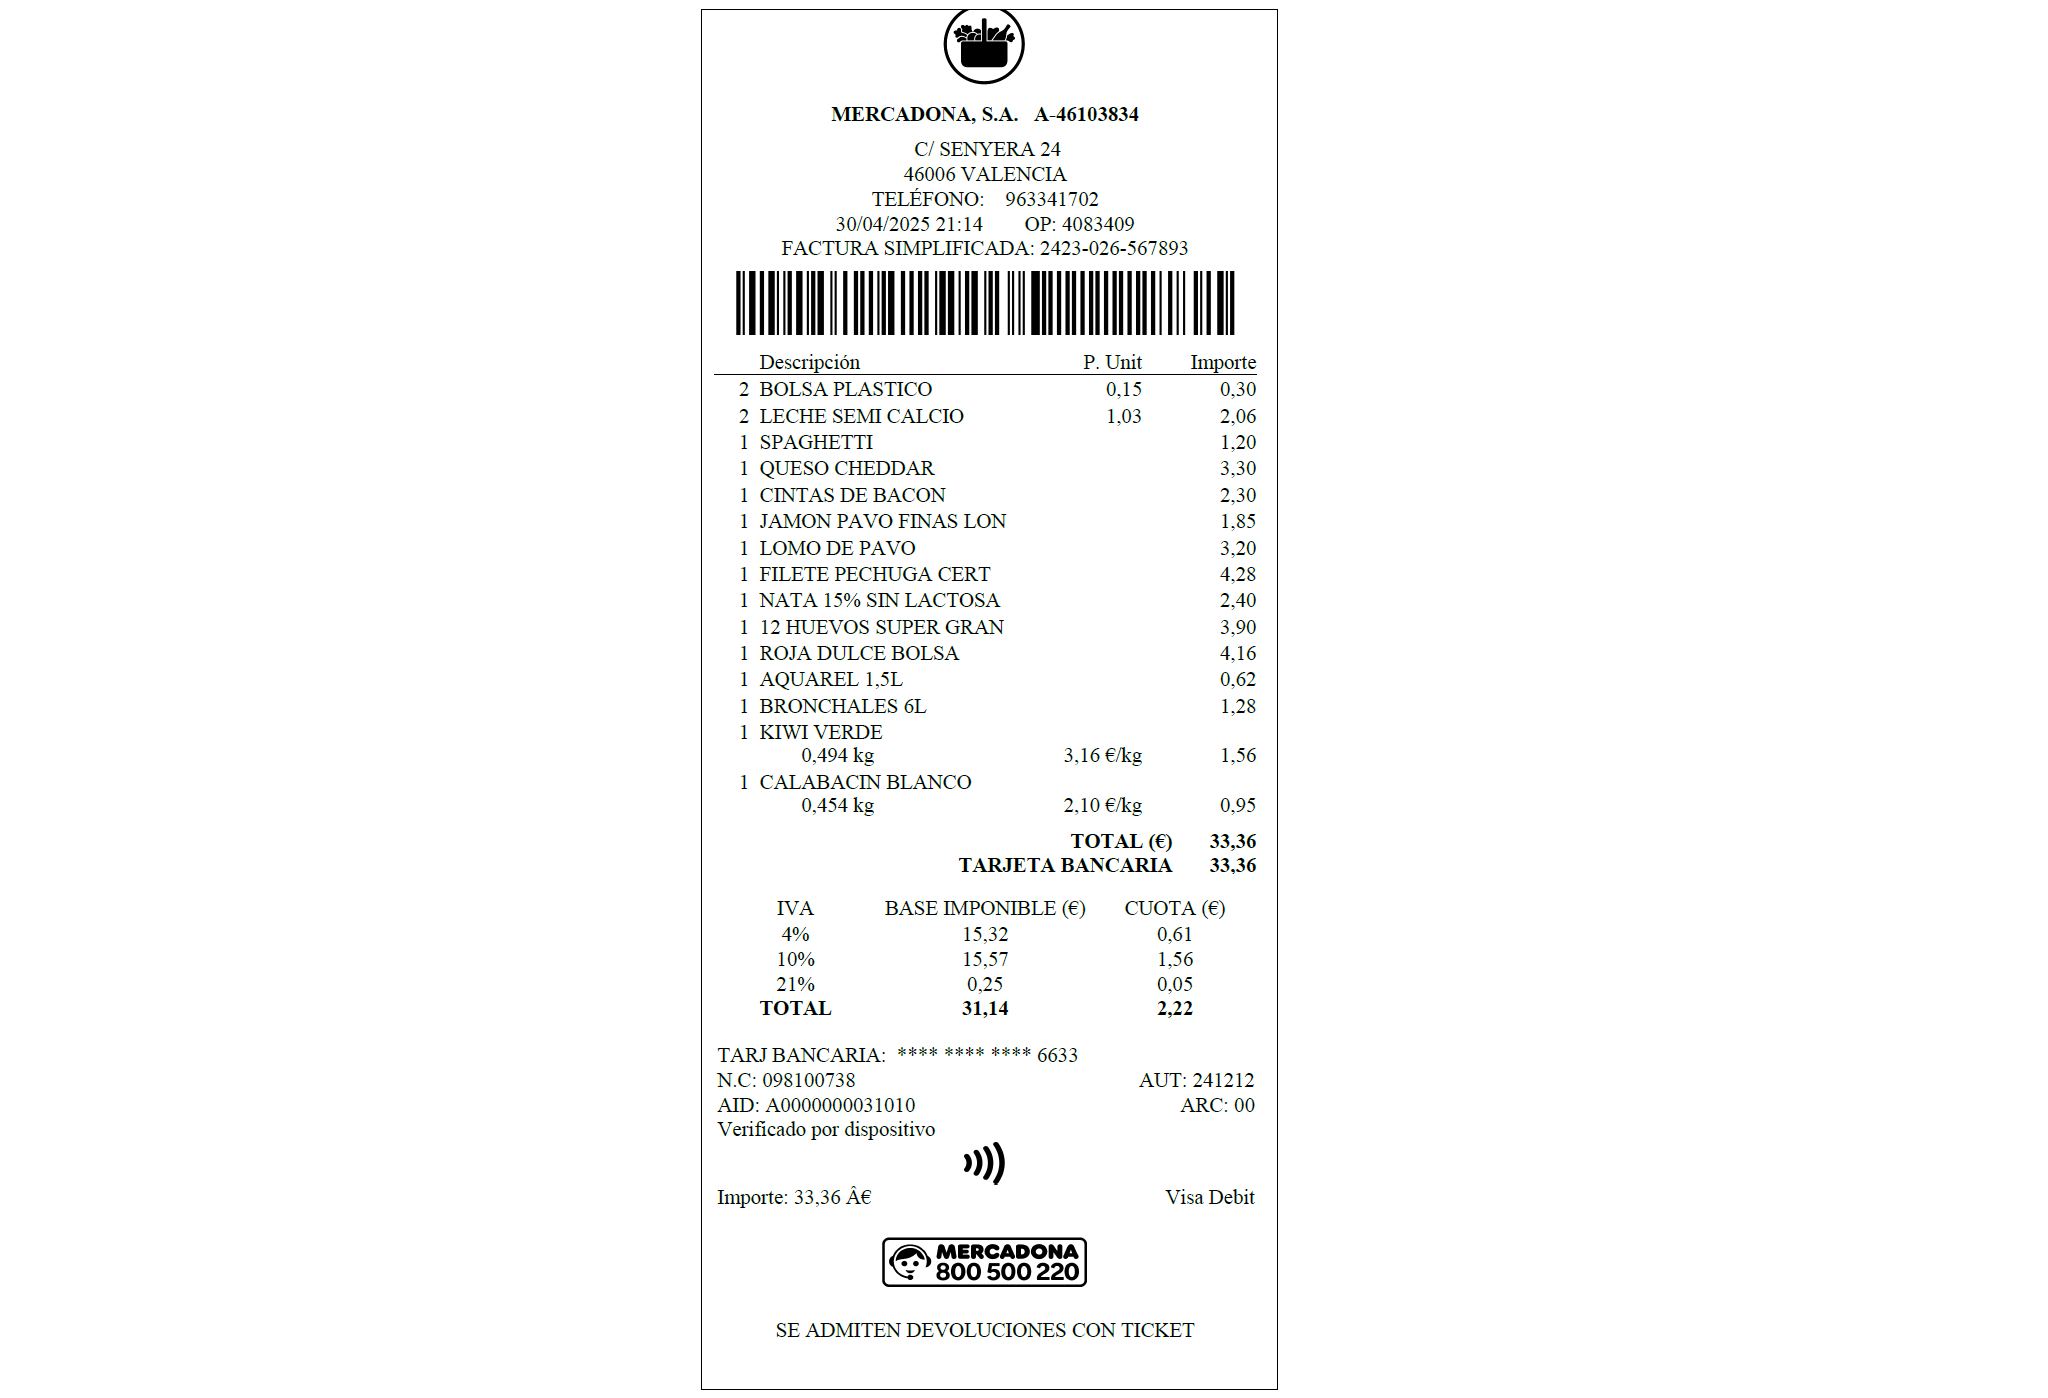
\includegraphics[width=1\linewidth]{imgEspecifiques/ticketExtraccioA.png}
				\label{fig:ticketExtraccioA}
			\end{figure}
		\end{frame}
		
	
		
		\begin{frame}
			\begin{figure}
				\centering
				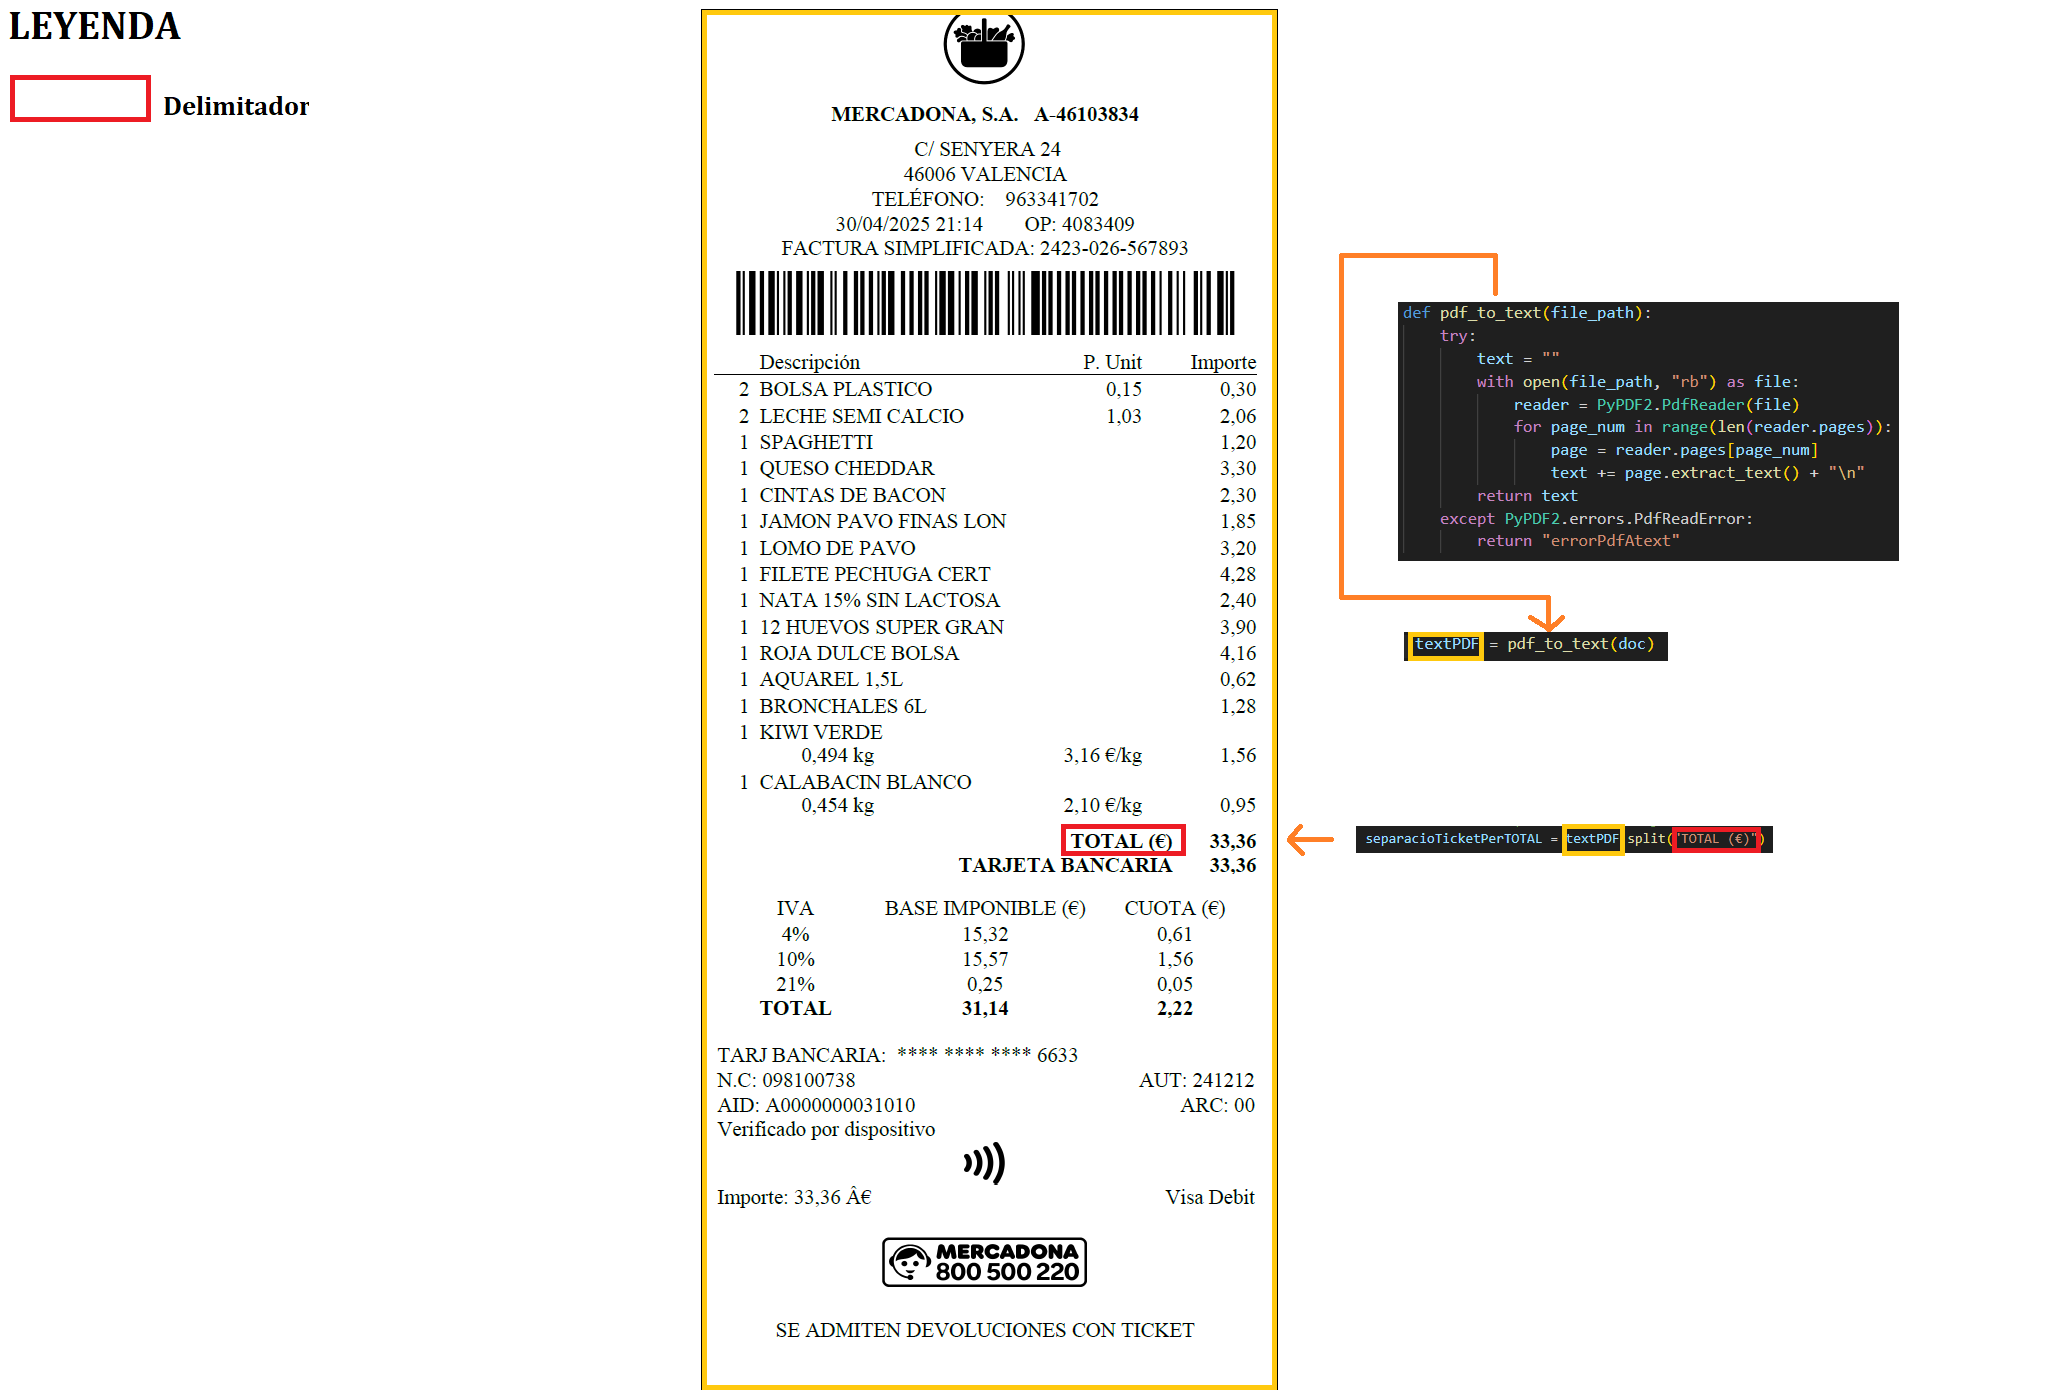
\includegraphics[width=1\linewidth]{imgEspecifiques/ticketExtraccioB.png}
				\label{fig:ticketExtraccioB}
			\end{figure}
		\end{frame}
		
		\begin{frame}
			\begin{figure}
				\centering
				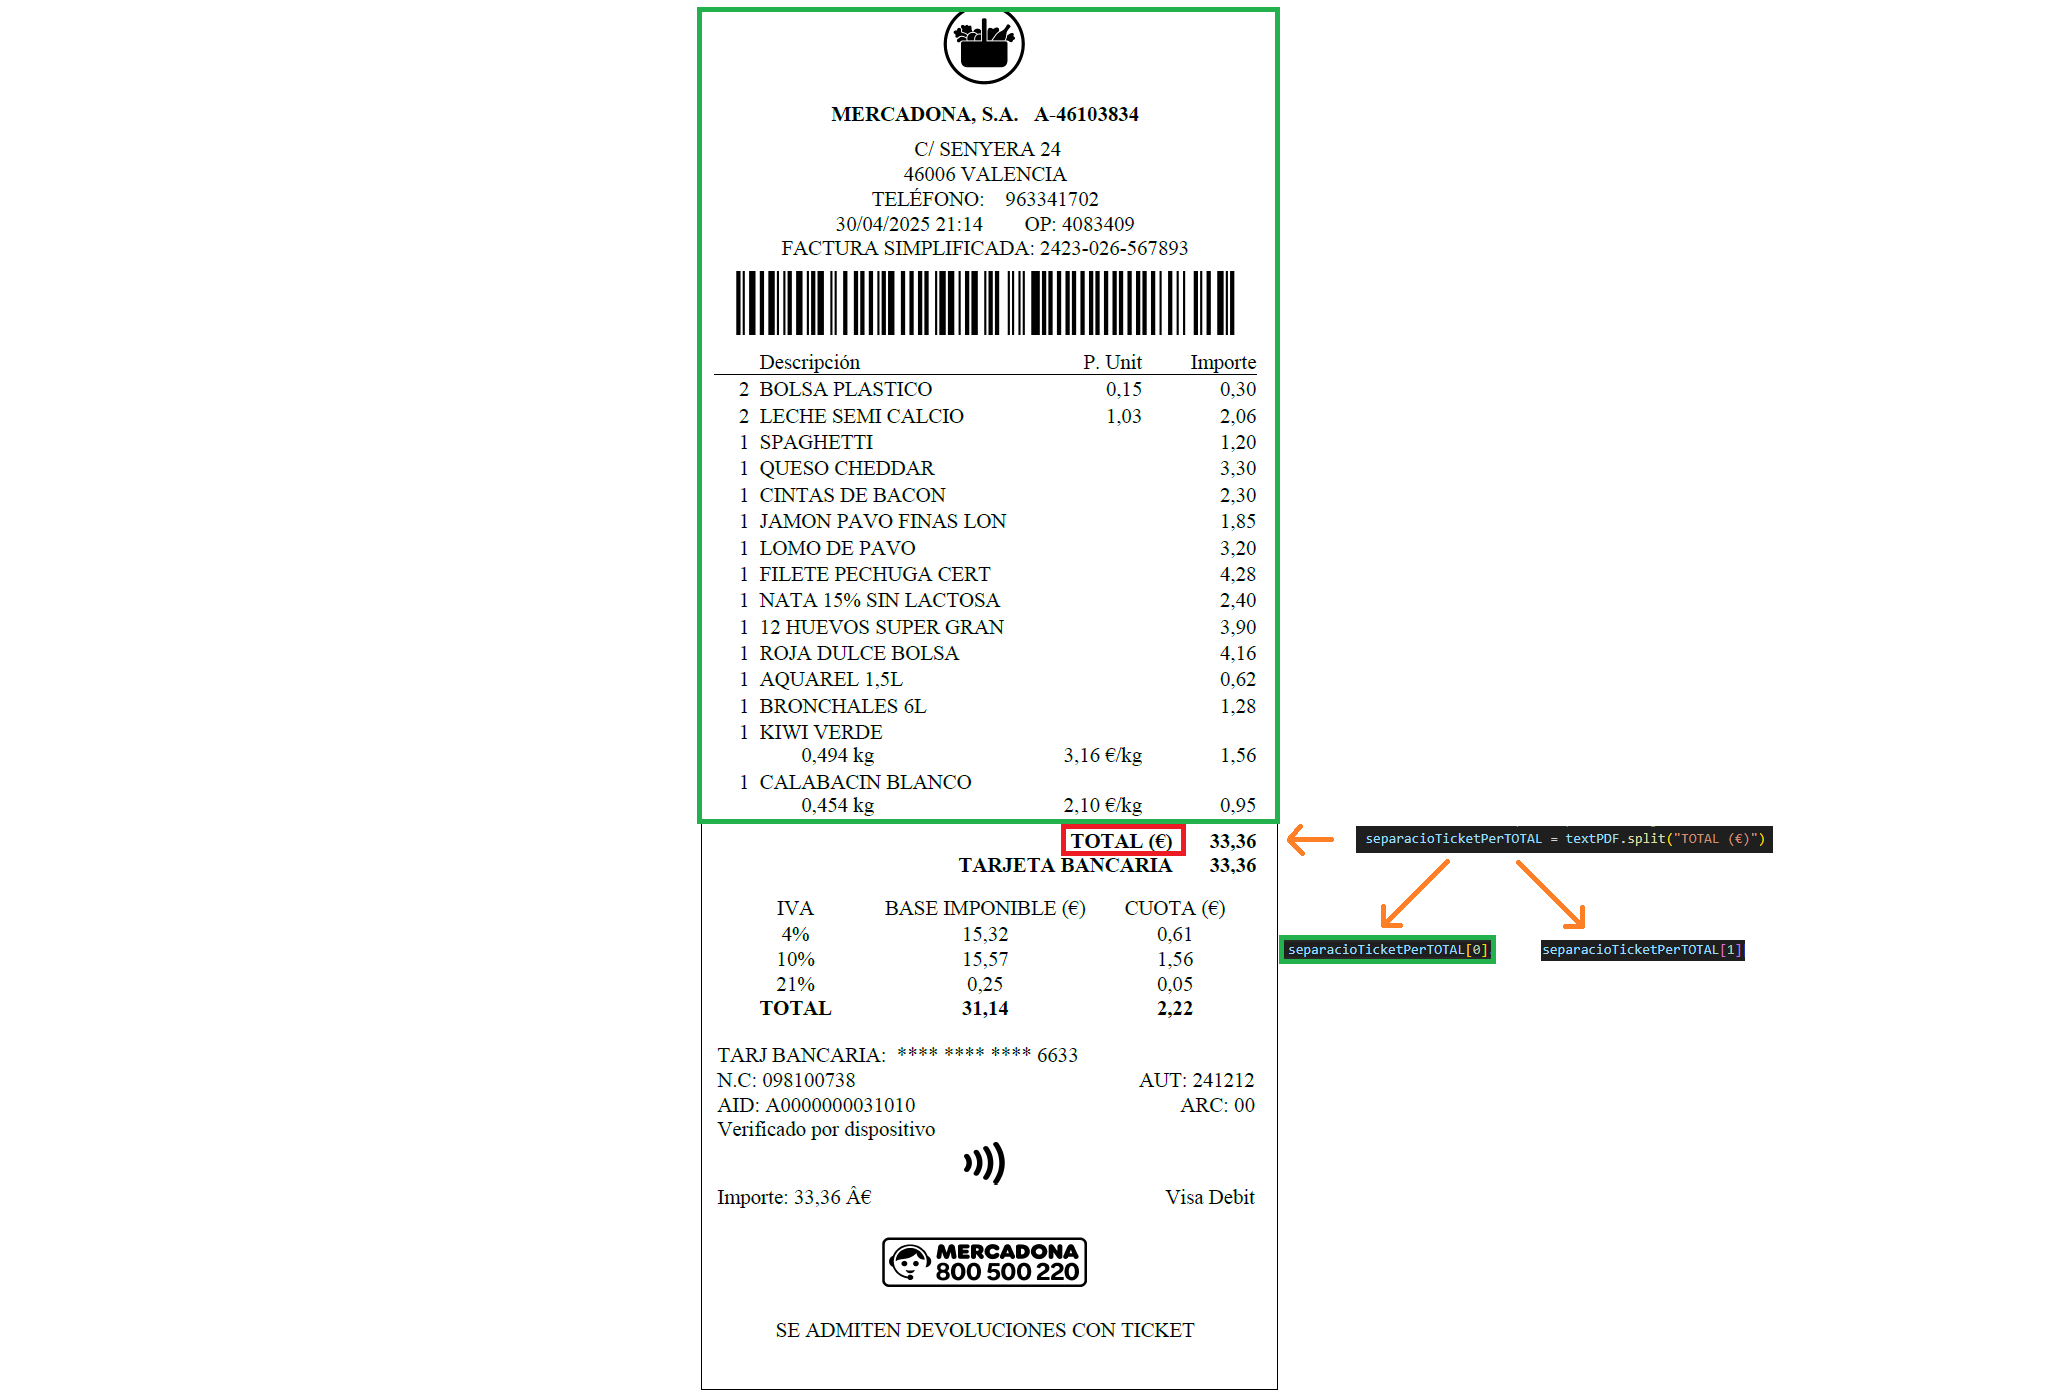
\includegraphics[width=1\linewidth]{imgEspecifiques/ticketExtraccioC.png}
				\label{fig:ticketExtraccioC}
			\end{figure}
		\end{frame}
		
		\begin{frame}
			\begin{figure}
				\centering
				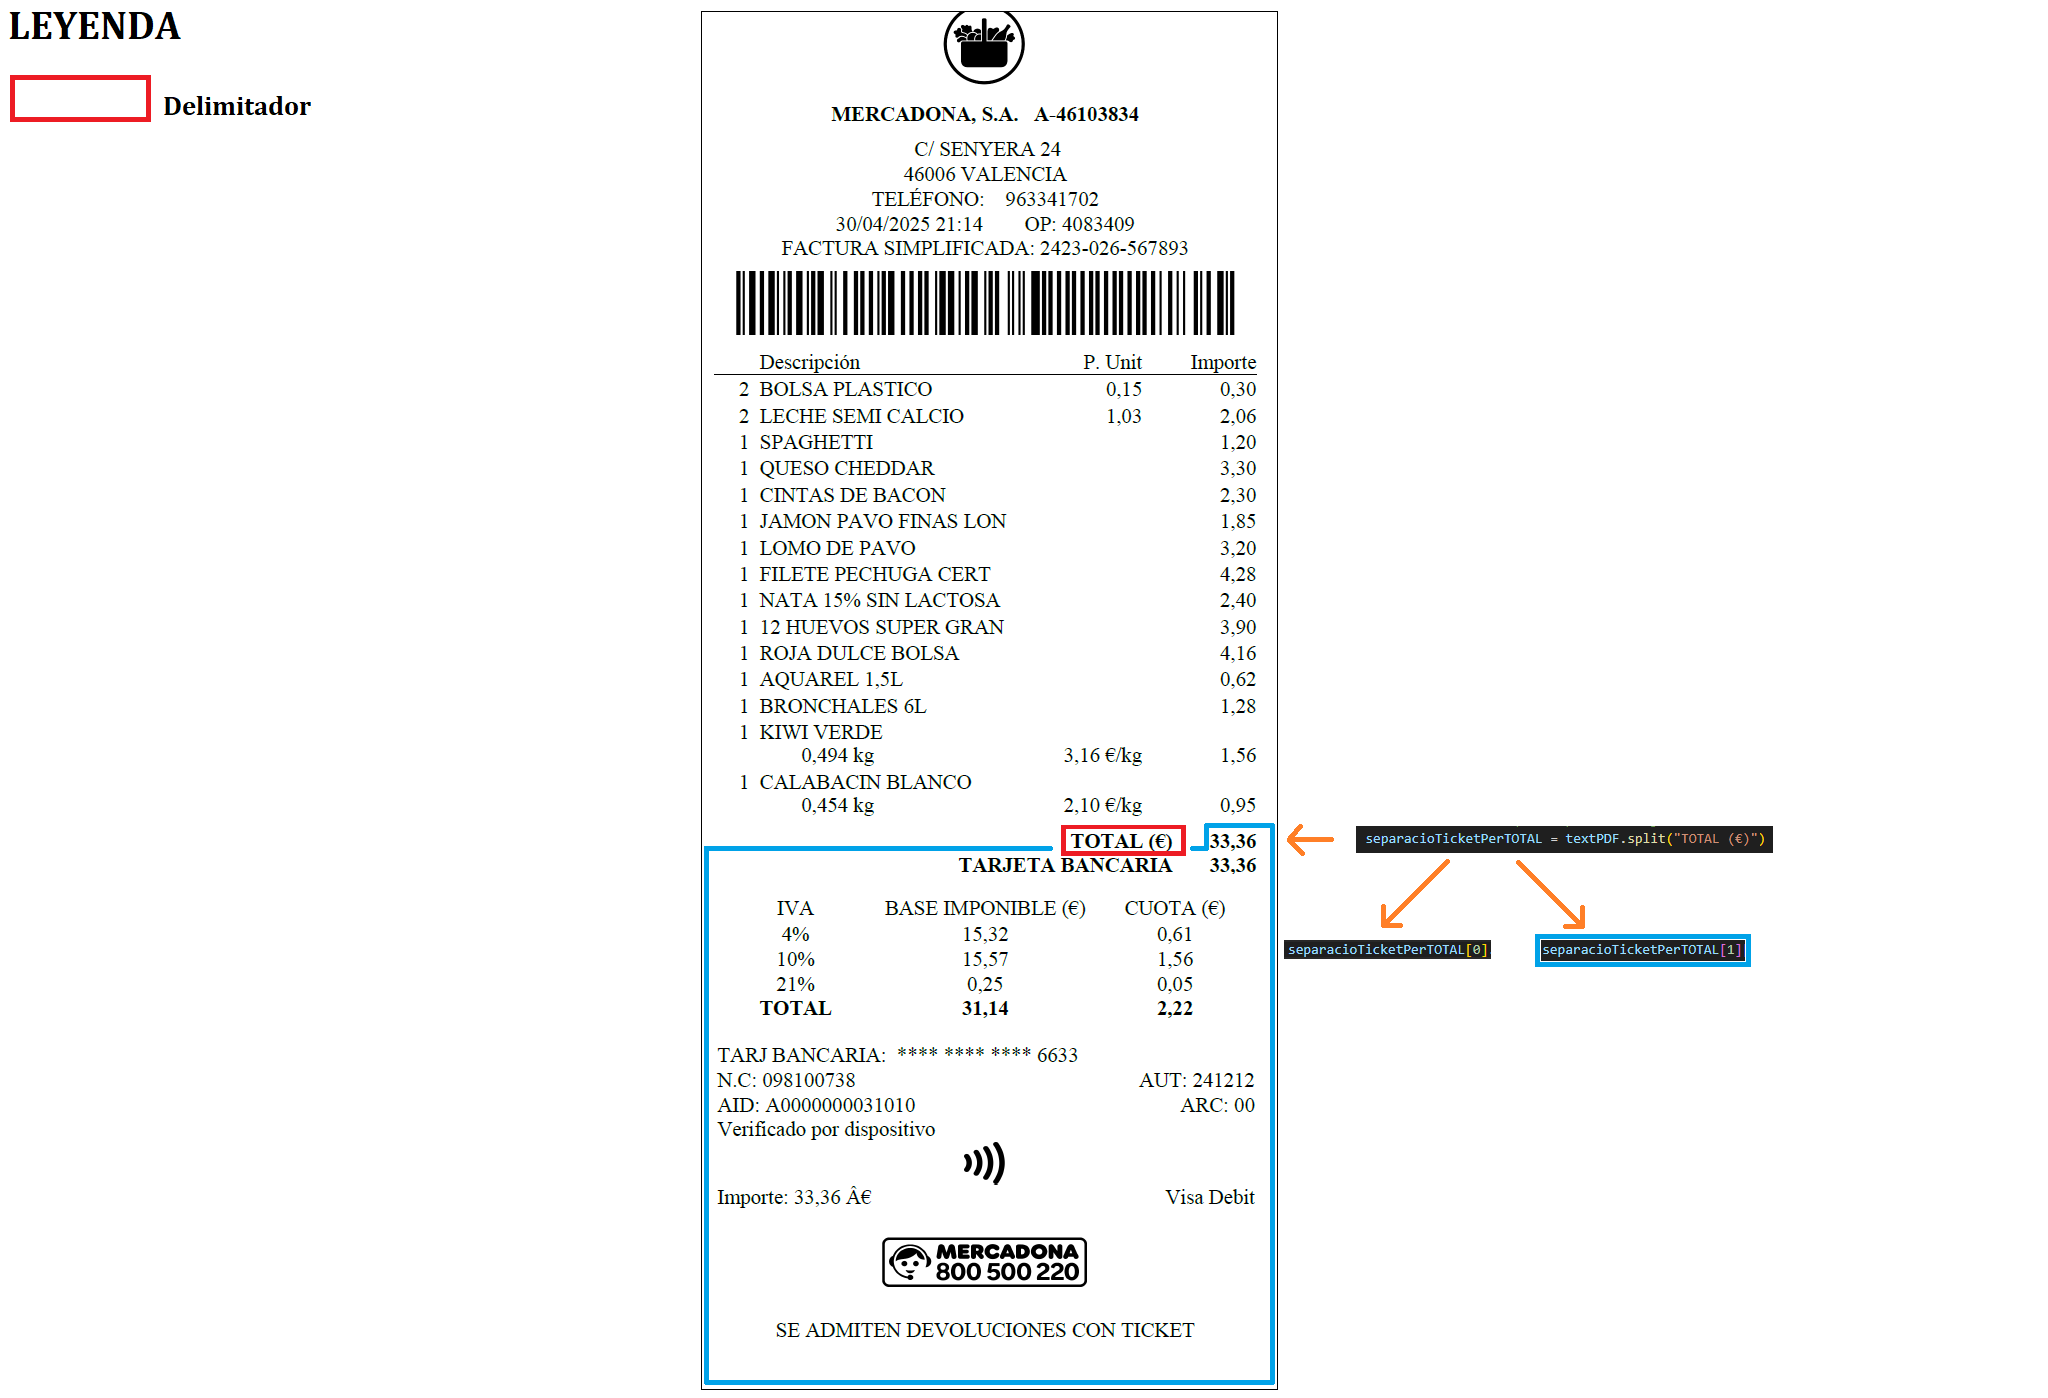
\includegraphics[width=1\linewidth]{imgEspecifiques/ticketExtraccioD.png}
				\label{fig:ticketExtraccioD}
			\end{figure}
		\end{frame}
		
		\begin{frame}
			\begin{figure}
				\centering
				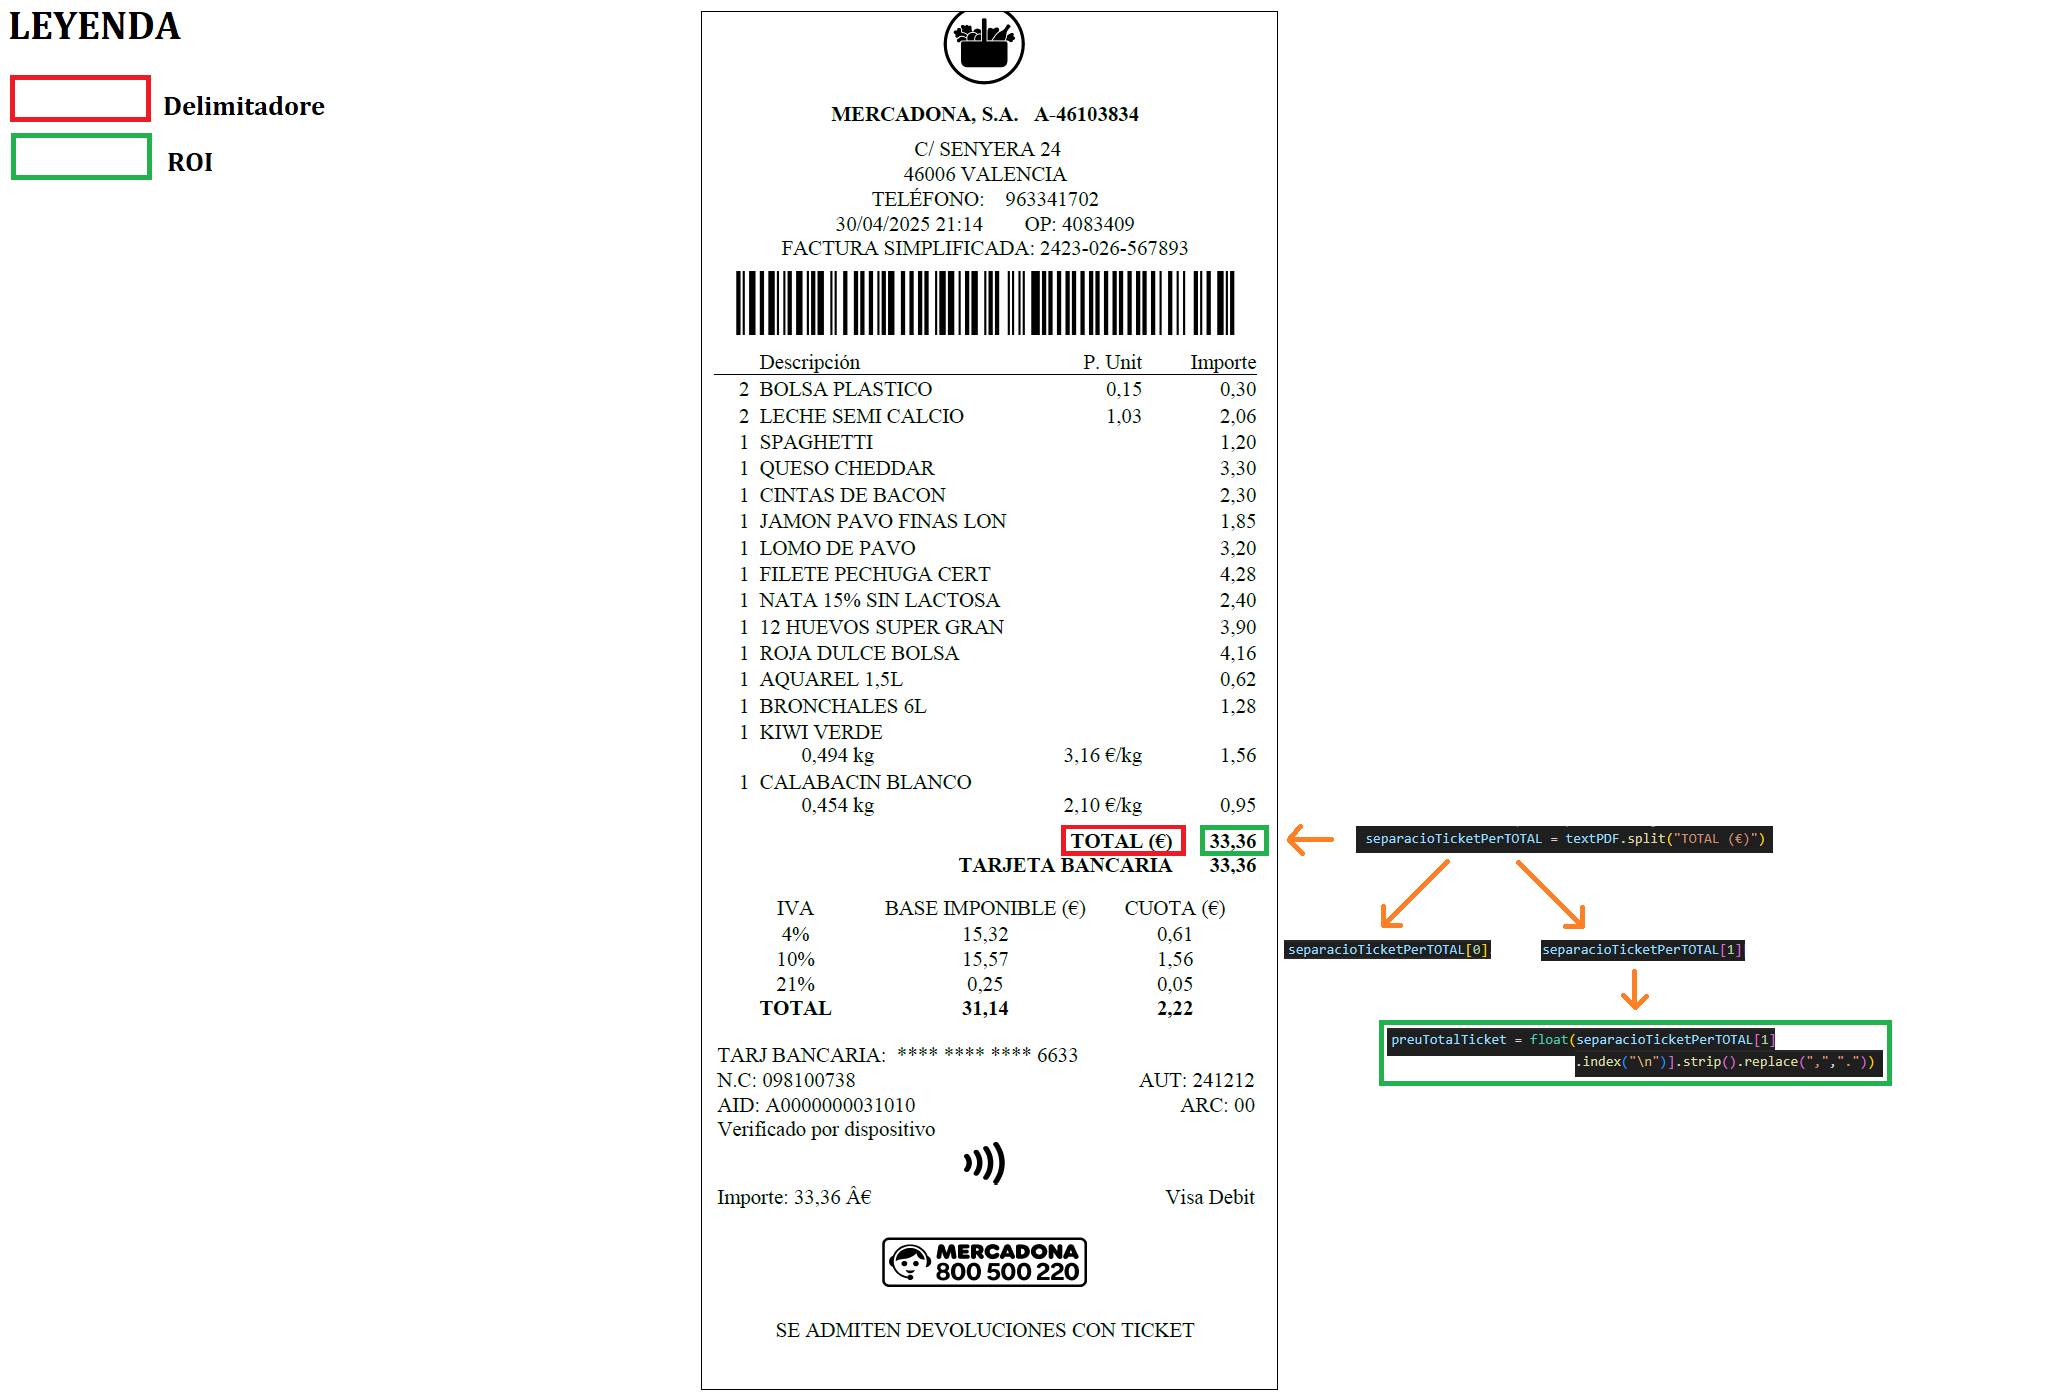
\includegraphics[width=1\linewidth]{imgEspecifiques/ticketExtraccioE.png}
				\label{fig:ticketExtraccioE}
			\end{figure}
		\end{frame}
		
		\begin{frame}
			\begin{figure}
				\centering
				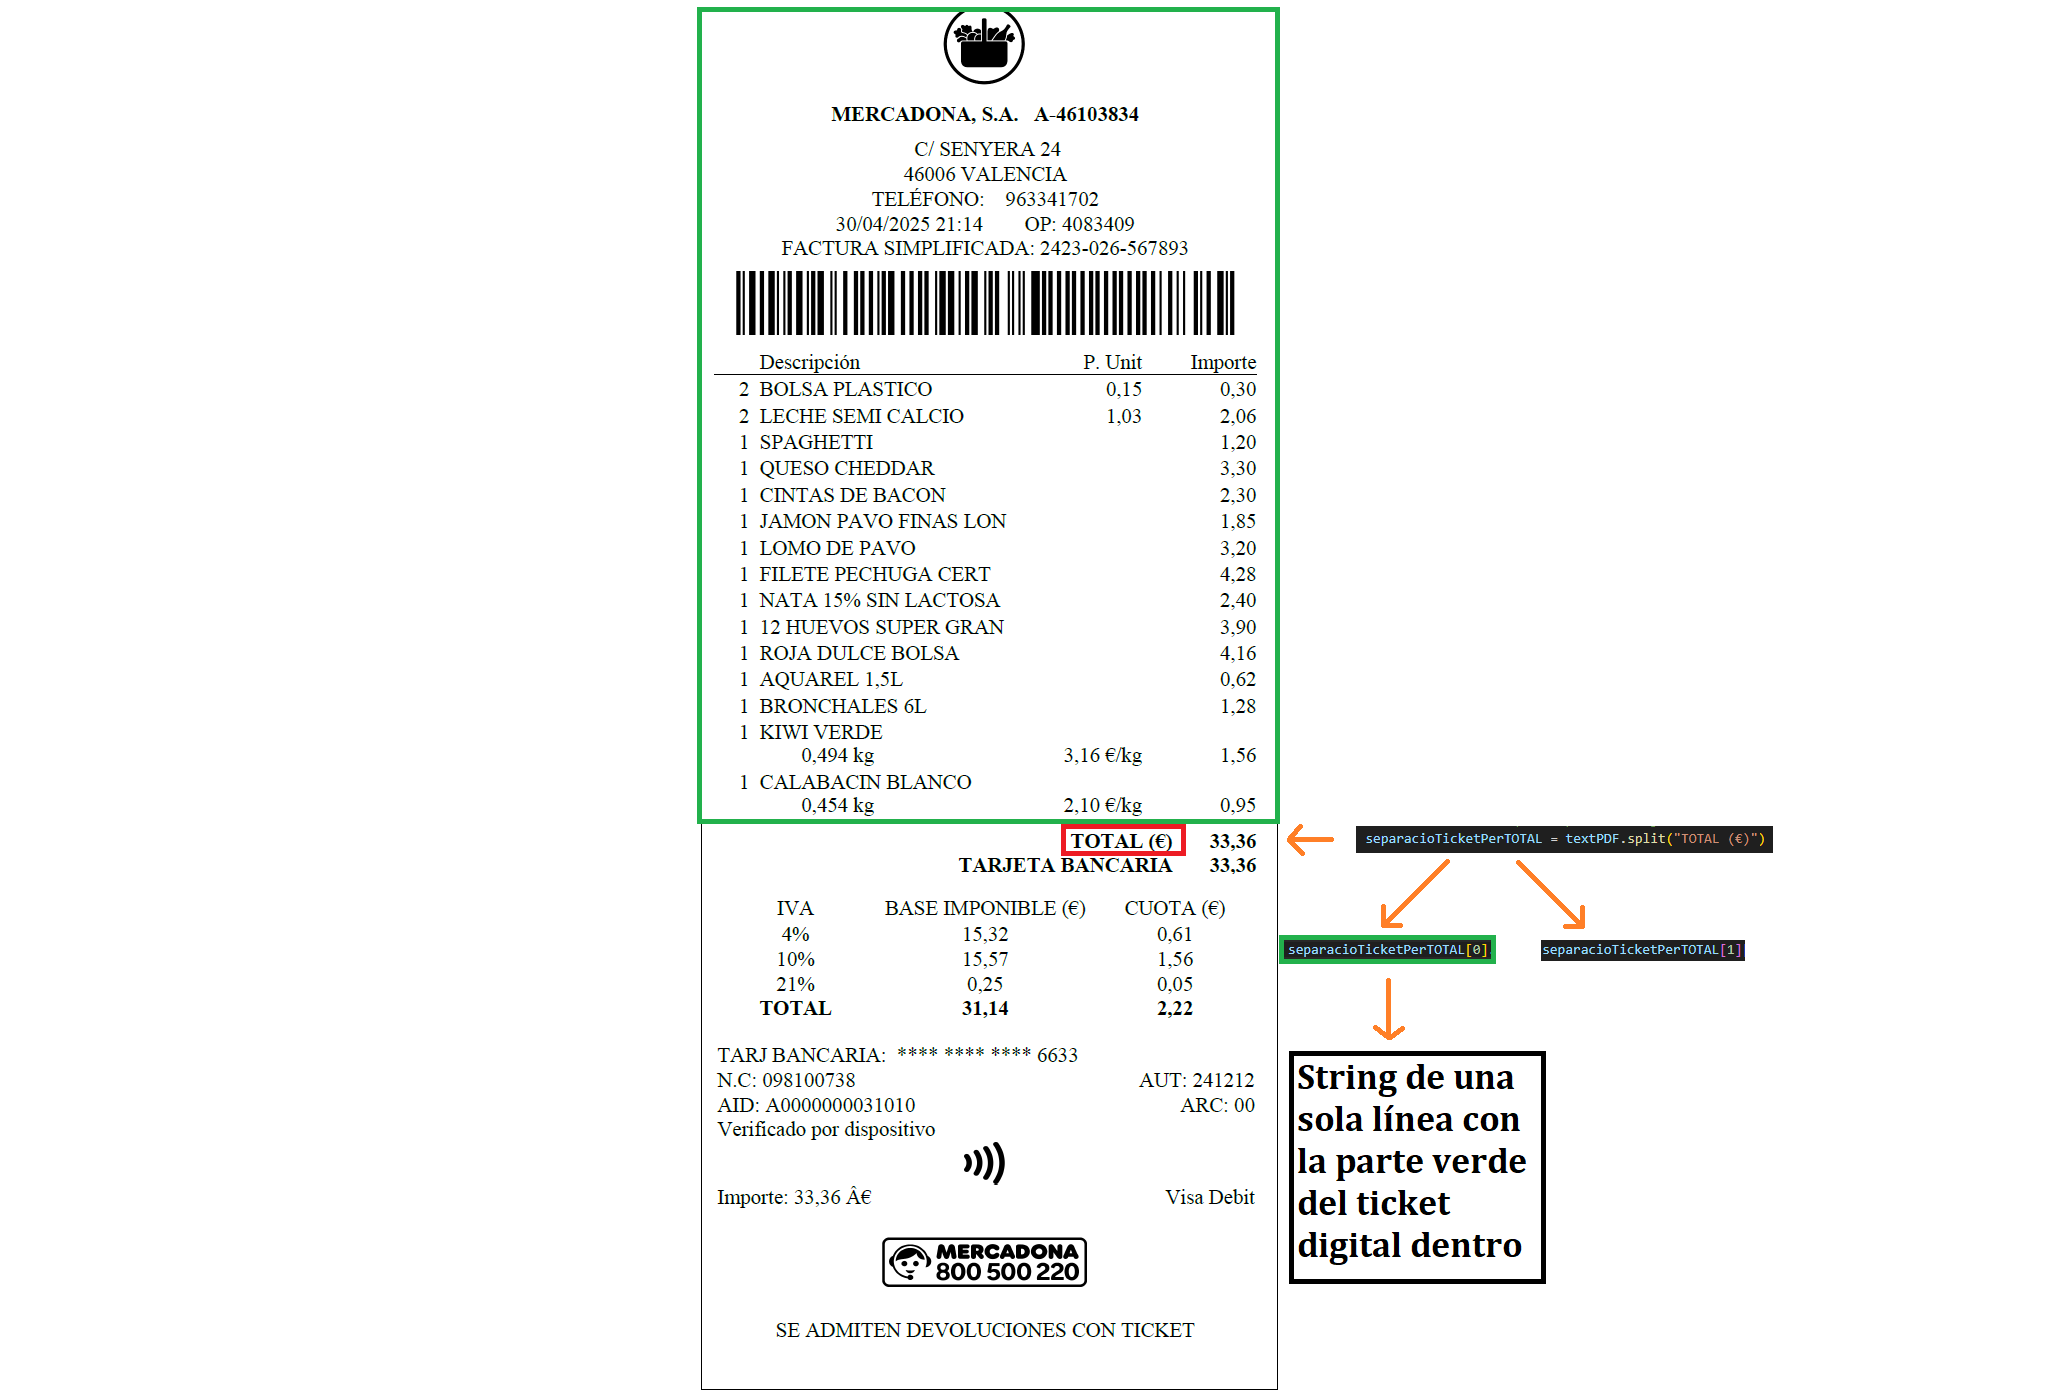
\includegraphics[width=1\linewidth]{imgEspecifiques/ticketExtraccioF.png}
				\label{fig:ticketExtraccioF}
			\end{figure}
		\end{frame}
		
		\begin{frame}
			\begin{figure}
				\centering
				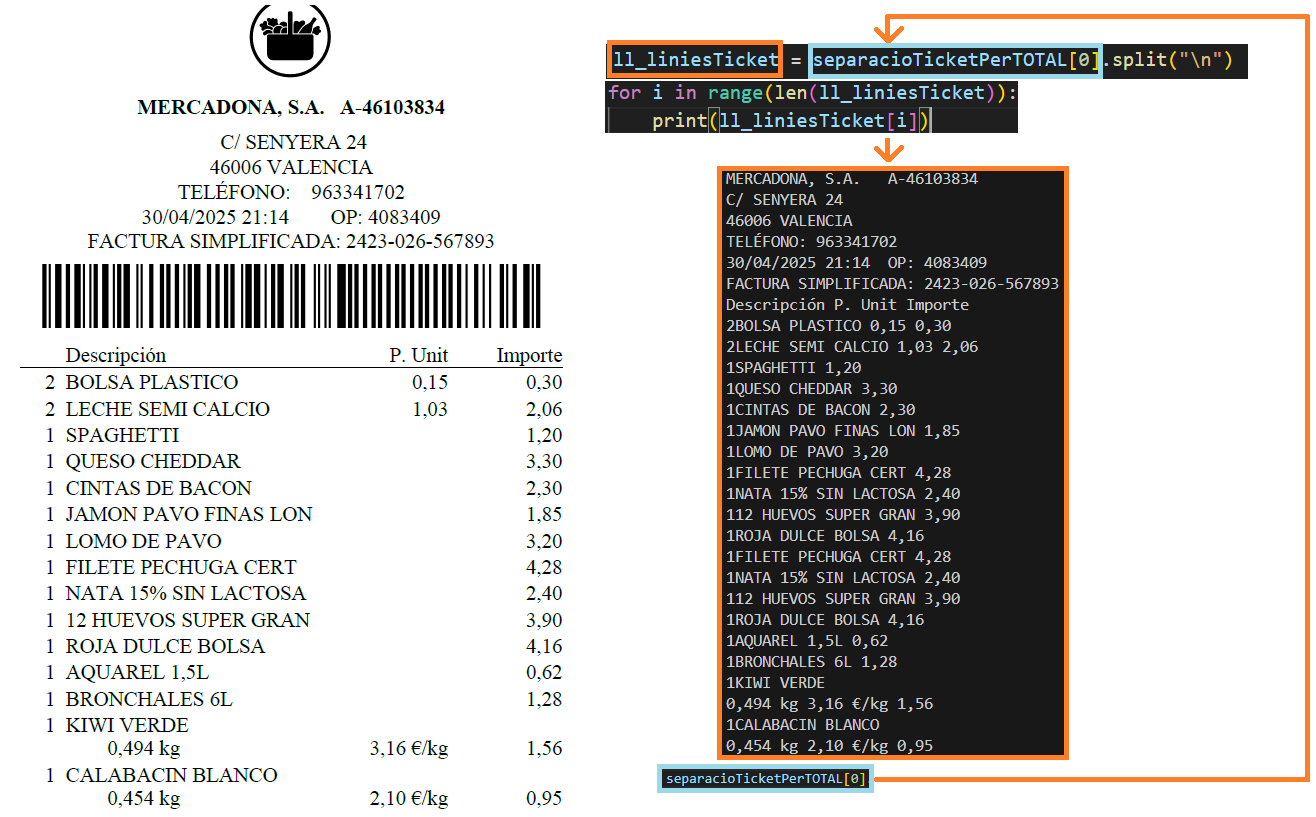
\includegraphics[width=1\linewidth]{imgEspecifiques/ticketExtraccioG.png}
				\label{fig:ticketExtraccioG}
			\end{figure}
		\end{frame}
		
	
				
		\begin{frame}
			\begin{figure}
				\centering
				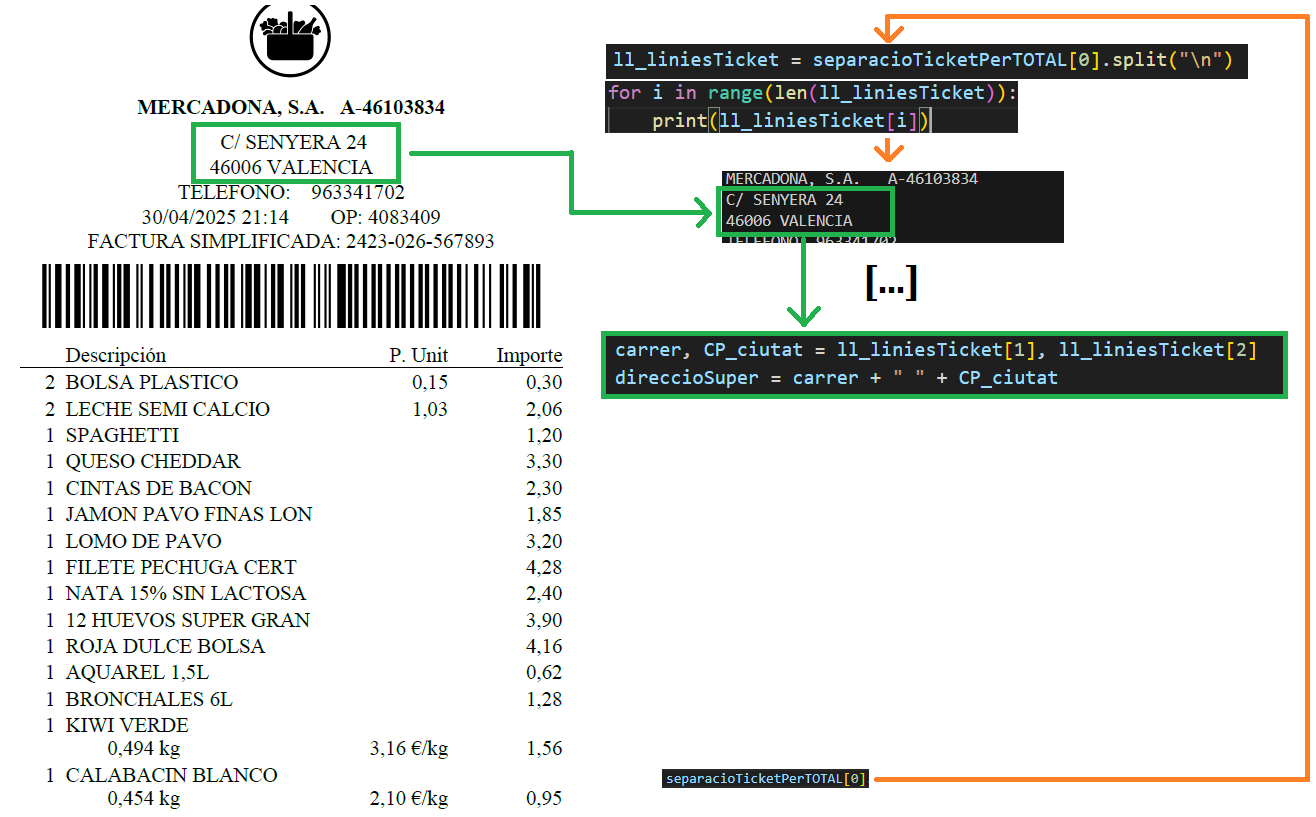
\includegraphics[width=1\linewidth]{imgEspecifiques/ticketExtraccioH.png}
				\label{fig:ticketExtraccioH}
			\end{figure}
		\end{frame}
		
		
		\begin{frame}
			\begin{figure}
				\centering
				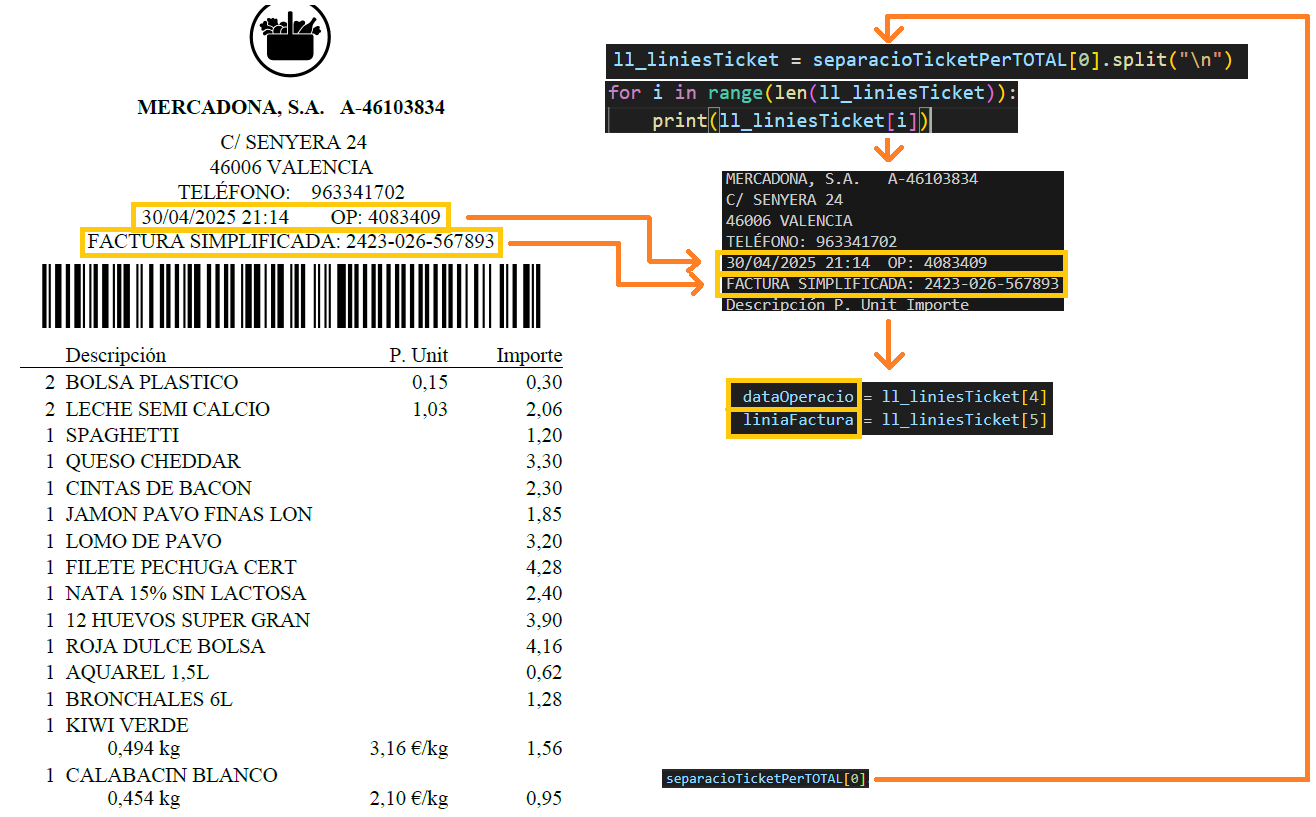
\includegraphics[width=1\linewidth]{imgEspecifiques/ticketExtraccioI.png}
				\label{fig:ticketExtraccioI}
			\end{figure}
		\end{frame}
		
		\begin{frame}
			\begin{figure}
				\centering
				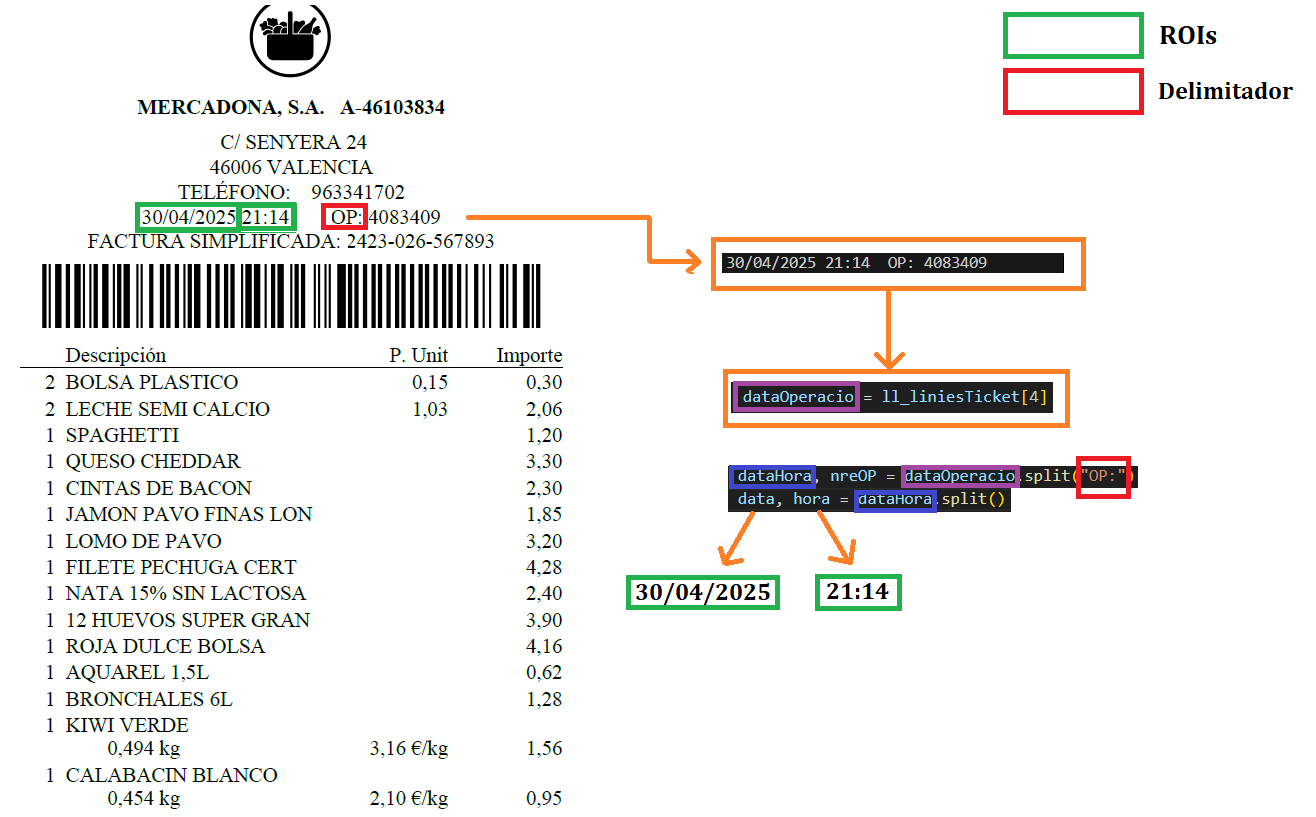
\includegraphics[width=1\linewidth]{imgEspecifiques/ticketExtraccioJ.png}
				\label{fig:ticketExtraccioJ}
			\end{figure}
		\end{frame}
		
		\begin{frame}
			\begin{figure}
				\centering
				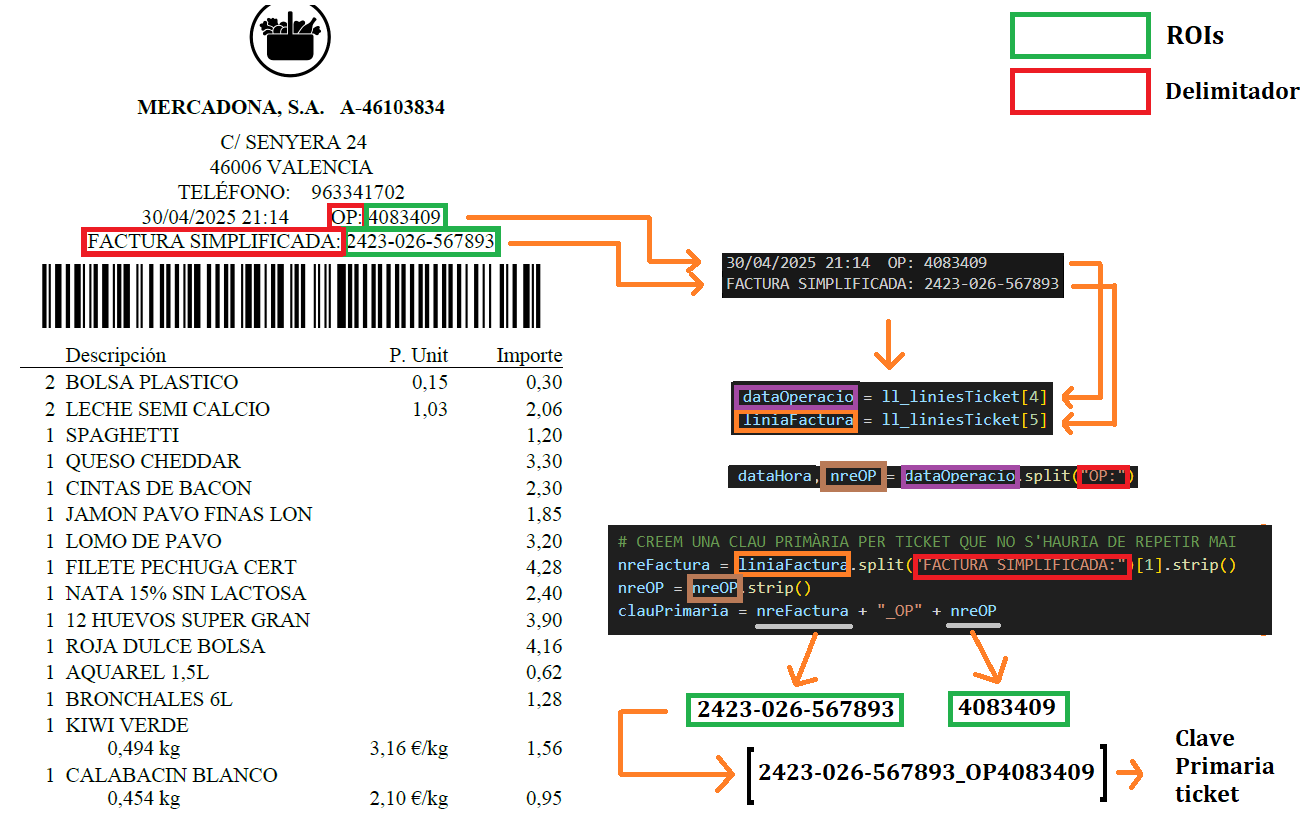
\includegraphics[width=1\linewidth]{imgEspecifiques/ticketExtraccioK.png}
				\label{fig:ticketExtraccioK}
			\end{figure}
		\end{frame}
			
	
			
		\begin{frame}
			\begin{figure}
				\centering
				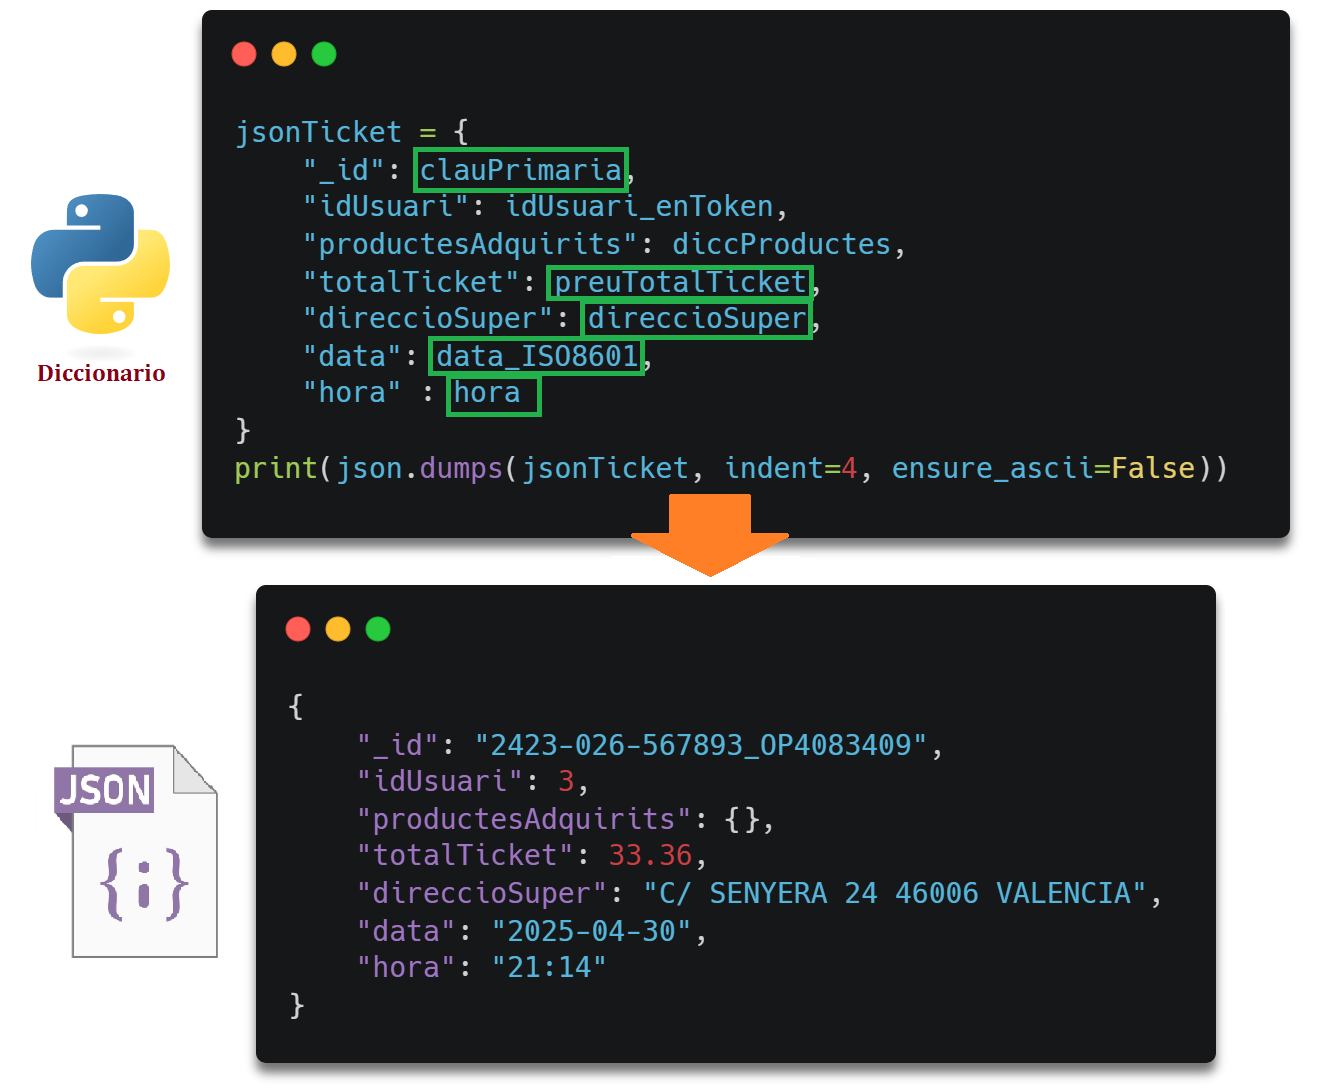
\includegraphics[width=.8\linewidth]{imgEspecifiques/ticketExtraccioL.png}
				\label{fig:ticketExtraccioL}
			\end{figure}
		\end{frame}
		
		\begin{frame}
			\begin{figure}
				\centering
				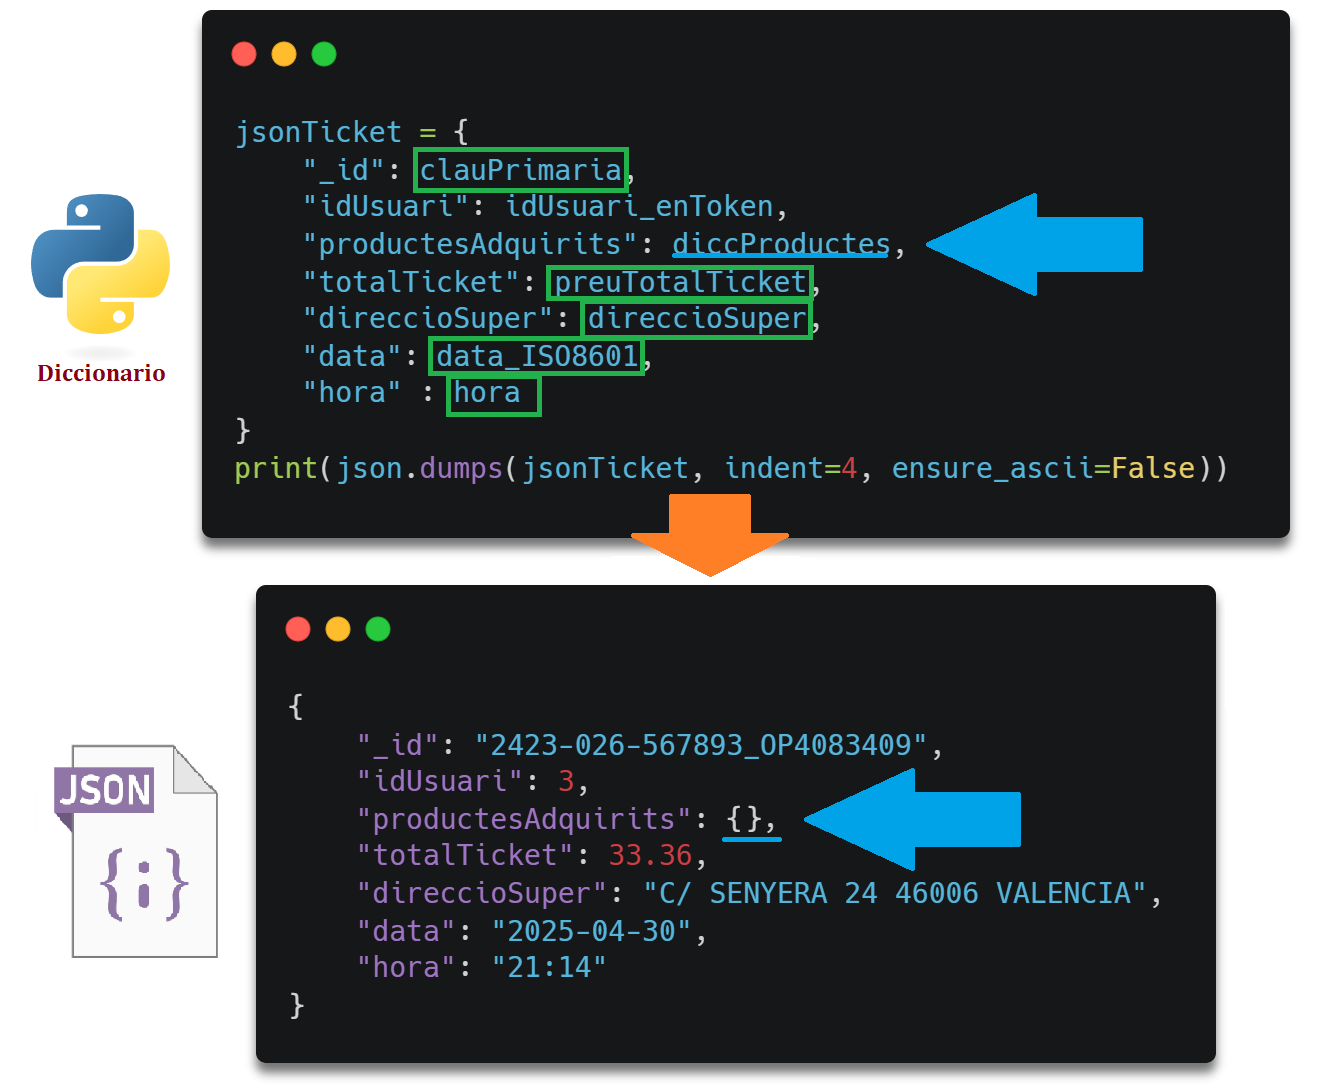
\includegraphics[width=.8\linewidth]{imgEspecifiques/ticketExtraccioM.png}
				\label{fig:ticketExtraccioM}
			\end{figure}
		\end{frame}
	
		% CONTINUAR FAST API AQUI
	
	
		\begin{frame}	
			\frametitle{1a Detección productos envasados}
			\begin{figure}
				\centering
				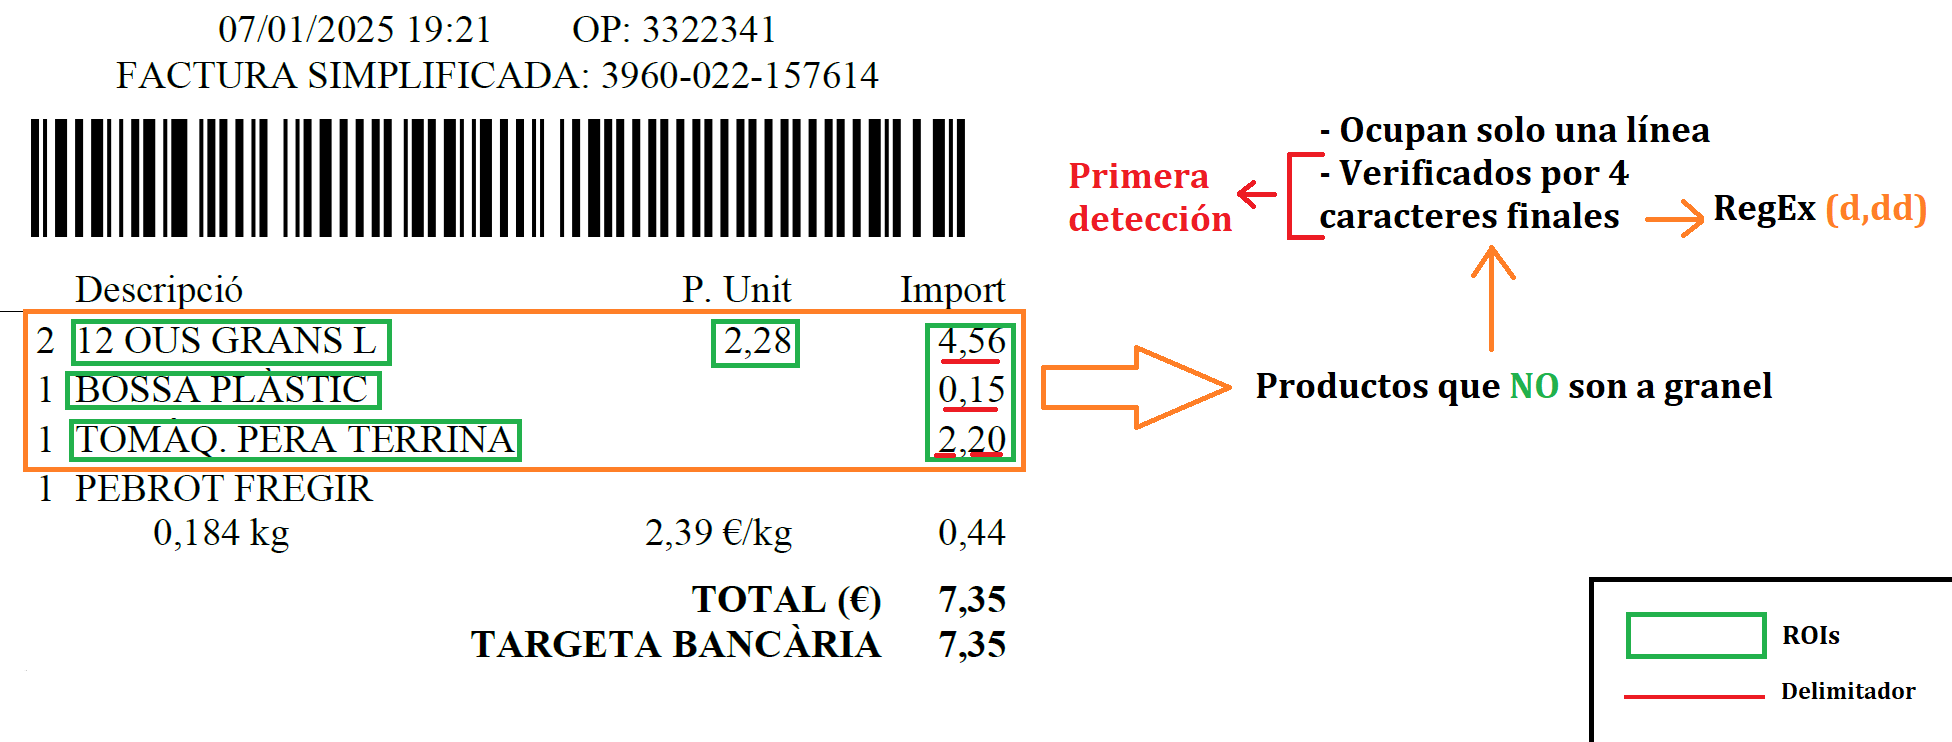
\includegraphics[width=1\linewidth]{imgEspecifiques/ticketExtraccioN1}
				\caption{Procedimiento: primera aproximación a la detección de productos que no son a granel mediante su importe.}
				\label{fig:ticketextraccionN1}
			\end{figure}
		\end{frame}
	
		\begin{frame}	
			\begin{figure}
				\frametitle{1a Detección productos a granel}
				\centering
				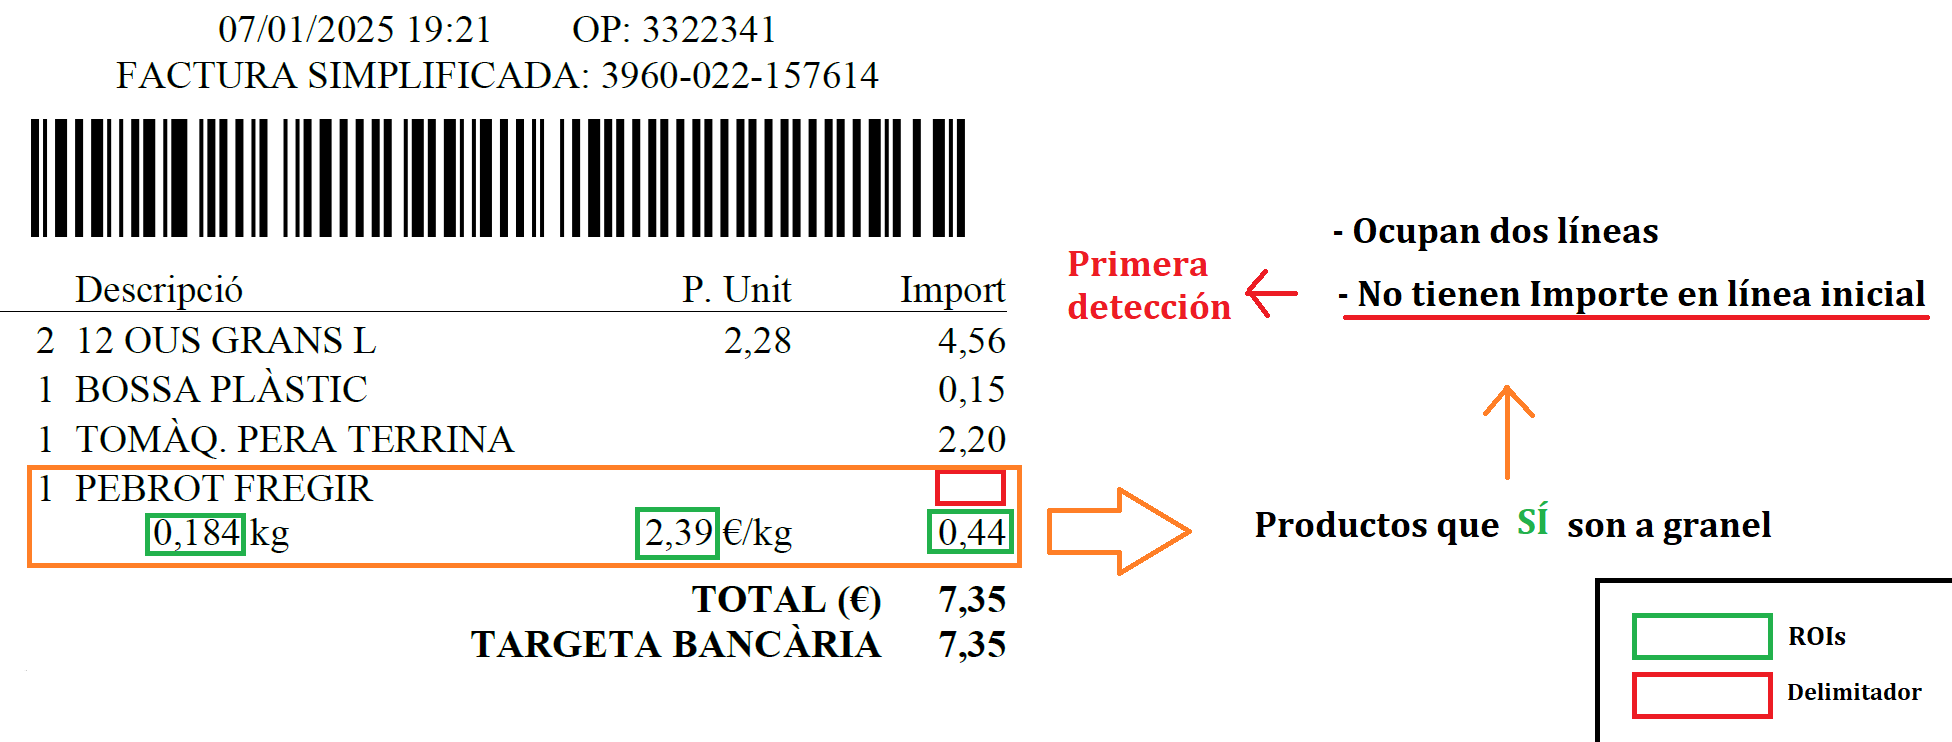
\includegraphics[width=1\linewidth]{imgEspecifiques/ticketExtraccioN2}
				\caption{Procedimiento: primera aproximación a la detección de productos a granel a partir de la falta de importe en su primera línea.}
				\label{fig:ticketextraccionN2}
			\end{figure}
		\end{frame}
	
	
	
	
		\begin{frame}	
			\begin{figure}
				\centering
				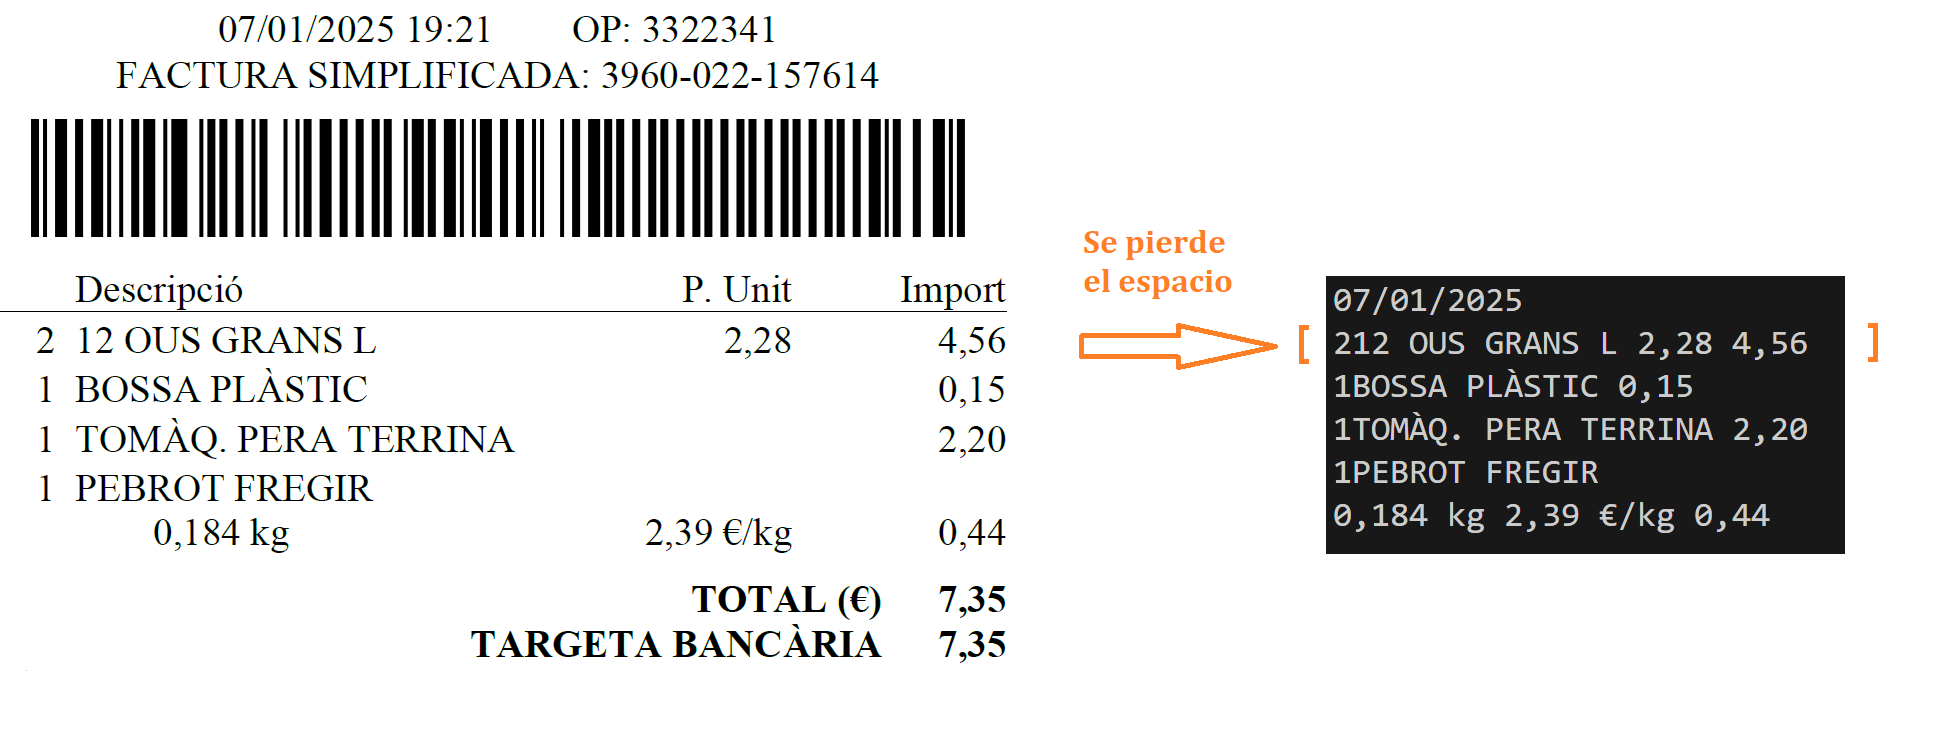
\includegraphics[width=1\linewidth]{imgEspecifiques/ticketExtraccioN}
				\caption{\textcolor{red}{producto conflictivo envasado}: número de unidades queda mezclado con el inicio de la descripción o nombre de un producto imposibilitando segmentar ambos datos mediante espacio (\textit{split()})}
				\label{fig:ticketextraccionN}
			\end{figure}
		\end{frame}
		
		
		\begin{frame}	
			\begin{figure}
				\centering
				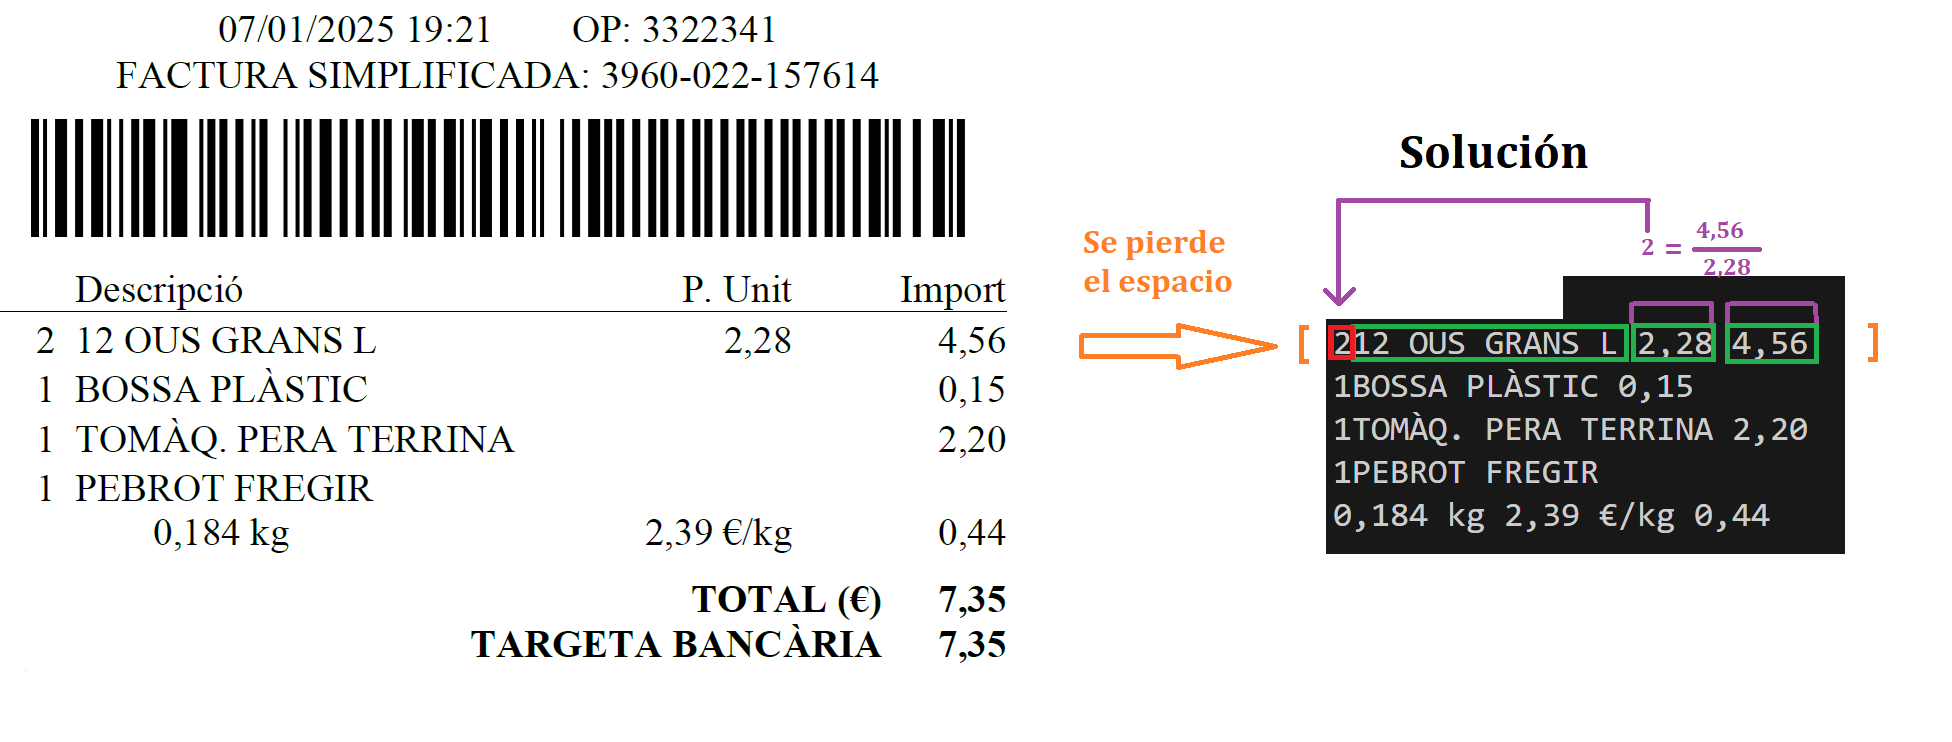
\includegraphics[width=1\linewidth]{imgEspecifiques/ticketExtraccioO}
				\caption{\textcolor{green}{Solución al conflicto}: se calcula qué parte de los dígitos pertenecen al número de unidades adquiridas y qué parte al nombre o descripción del mismo mediante coociente Importe/precioUnitario}
				\label{fig:ticketextraccionO}
			\end{figure}
		\end{frame}
			
			
	
	\begin{frame}	
		\begin{figure}
			\centering
			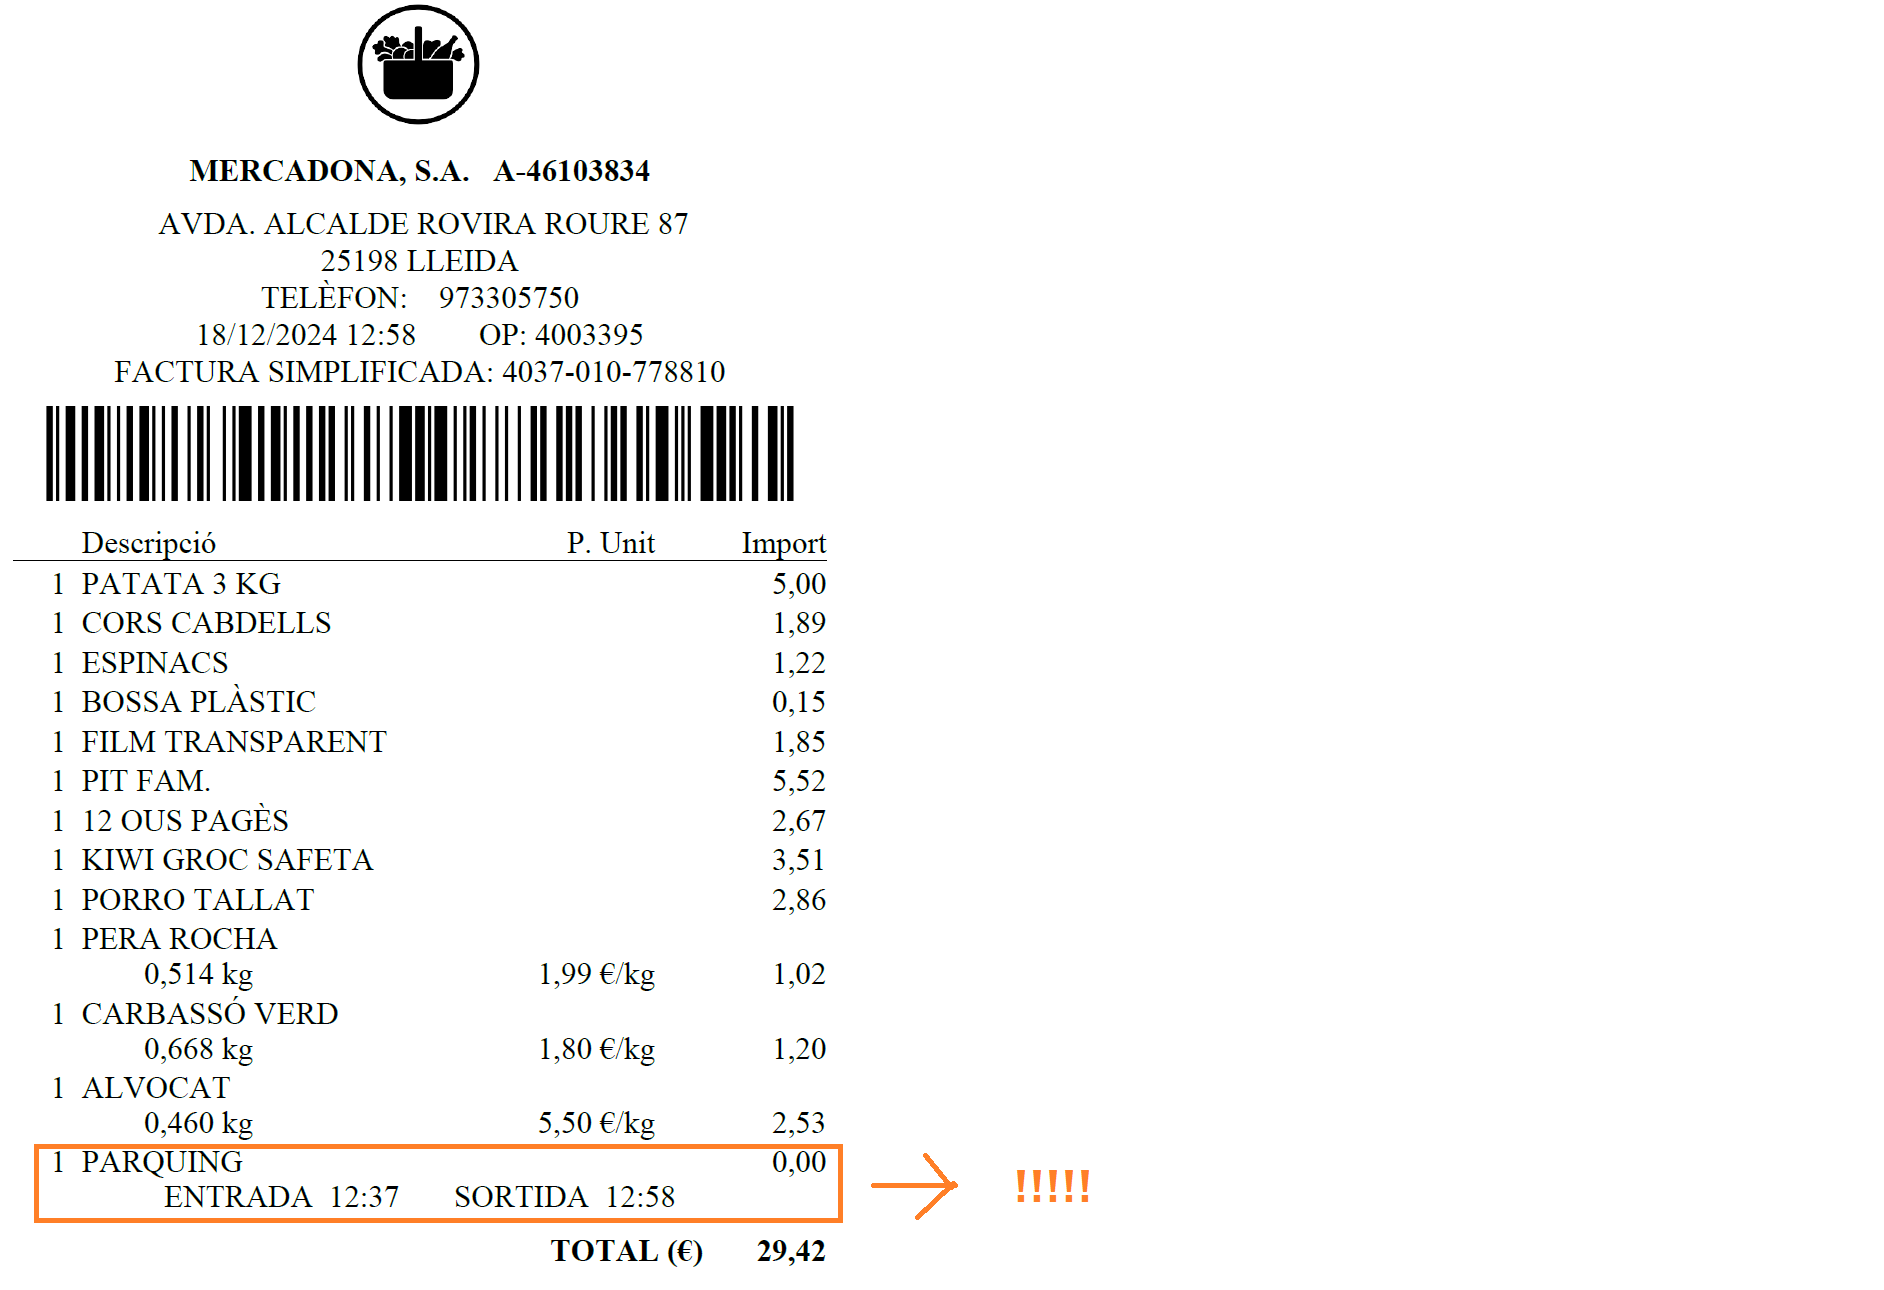
\includegraphics[width=.75\linewidth]{imgEspecifiques/ticketExtraccioP}
			\caption{\textcolor{red}{producto conflictivo}: Sale un parking que podemos confundir por un producto envasado (primera línea) y uno a granel (2a línea) que no tendría la línea que lo suele seguir con los datos a extraer.}
			\label{fig:ticketextraccionP}
		\end{figure}
	\end{frame}
	
	
	\begin{frame}	
		\begin{figure}
			\centering
			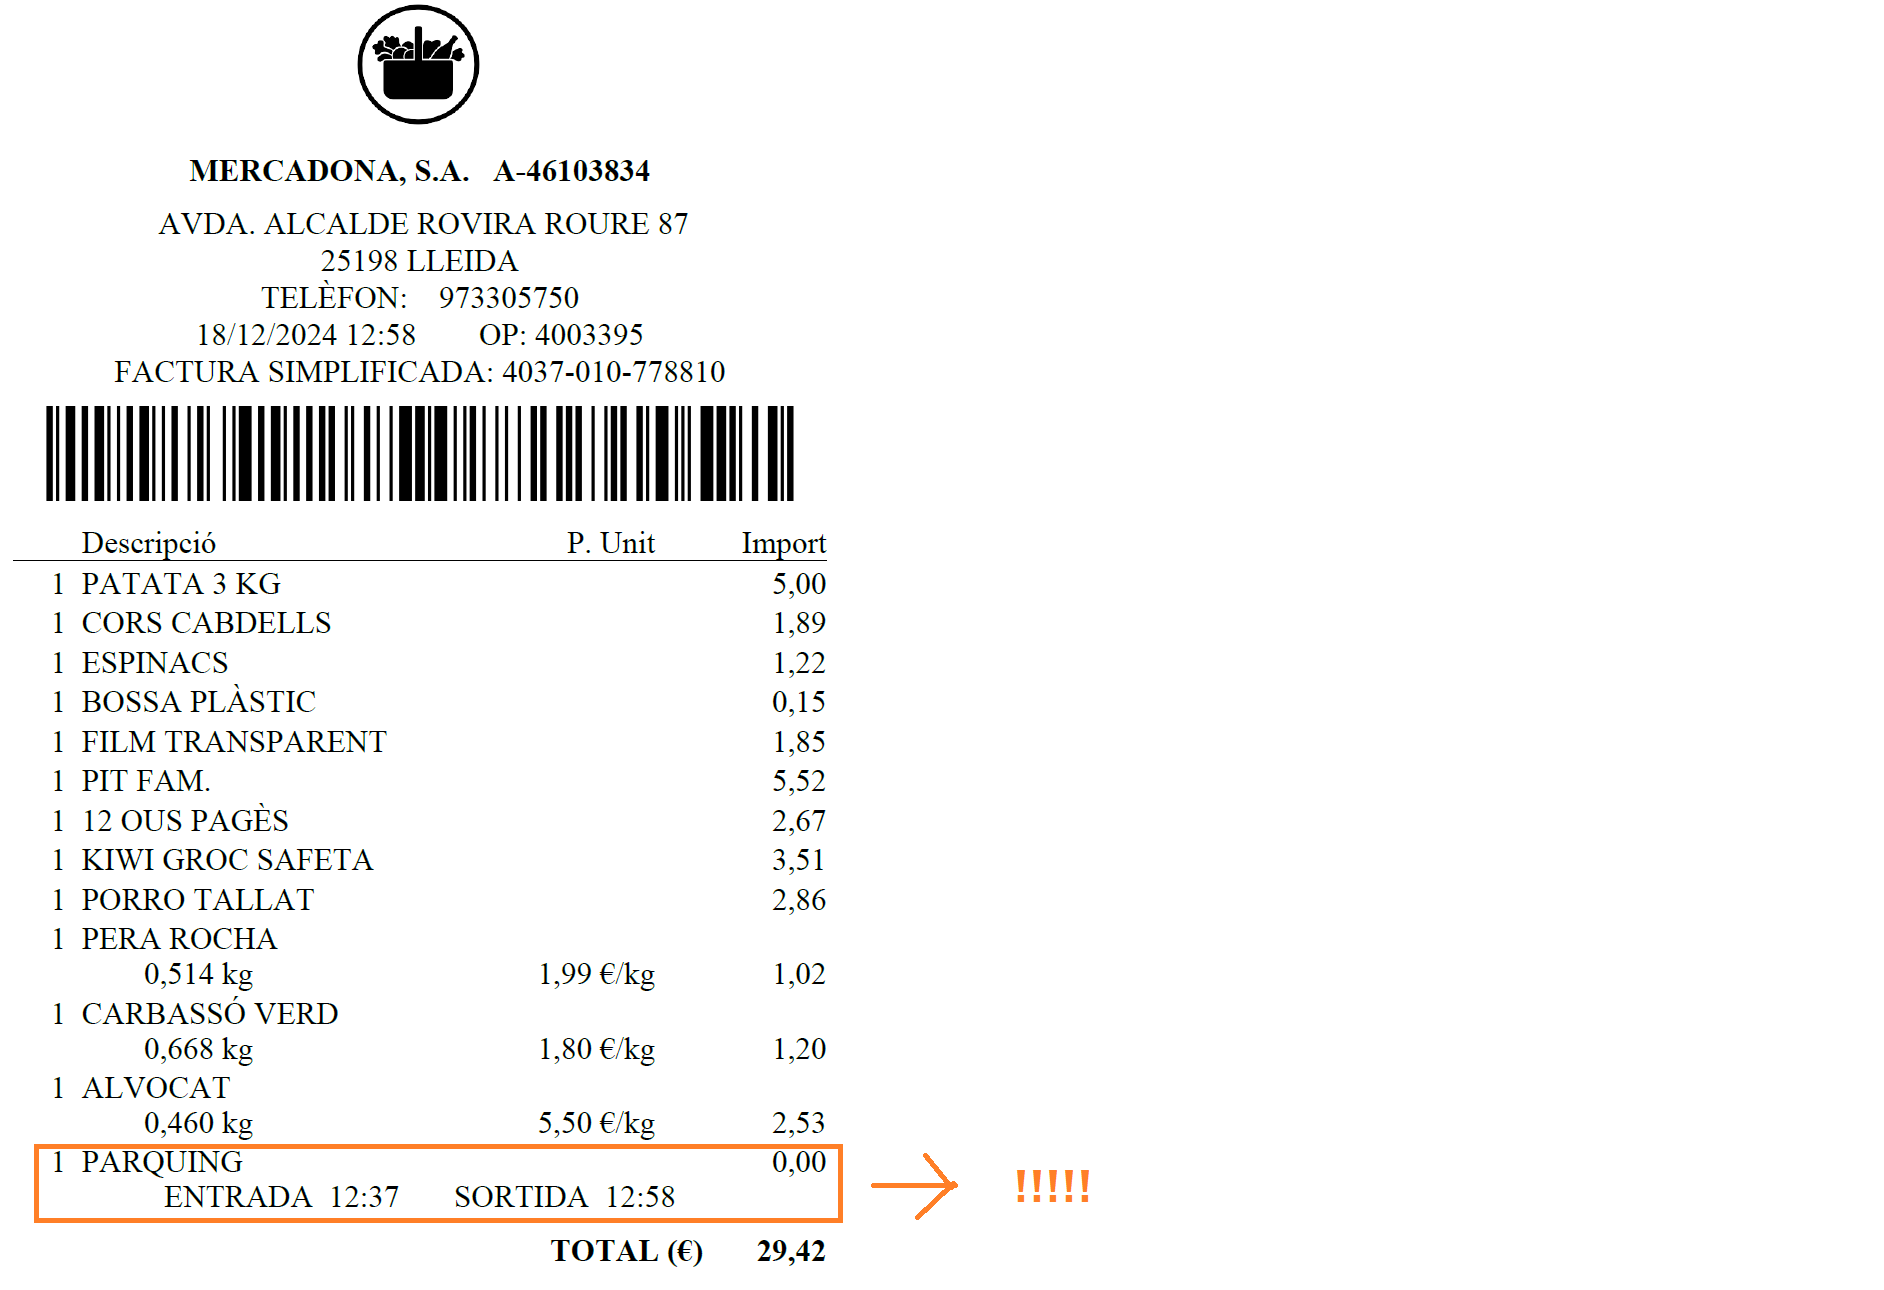
\includegraphics[width=.75\linewidth]{imgEspecifiques/ticketExtraccioQ}
			\caption{\textcolor{green}{Solución al conflicto}: Saltamos la línea que contiene "PARKING" y la siguiente}
			\label{fig:ticketextraccionQ}
		\end{figure}
	\end{frame}
	
	
	\begin{frame}
		\begin{figure}
			\centering
			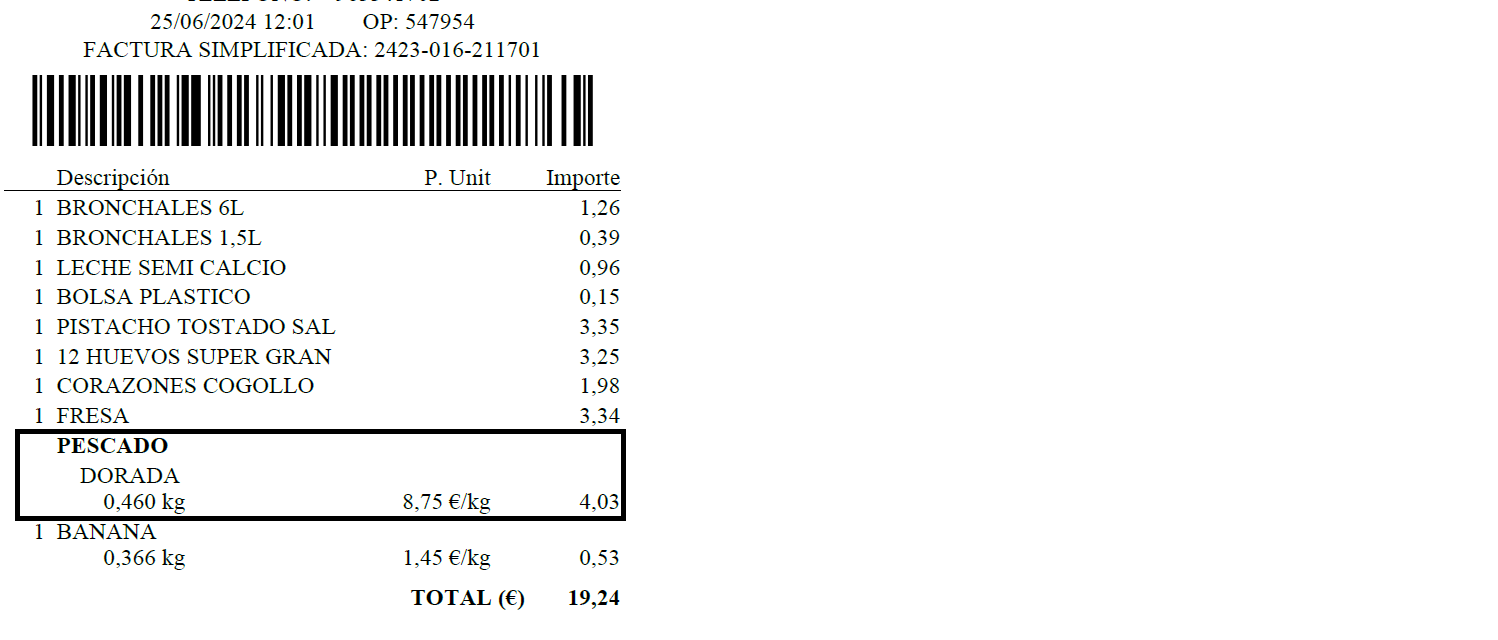
\includegraphics[width=1\linewidth]{imgEspecifiques/ticketExtraccioR}
			\caption{\textcolor{red}{producto conflictivo a granel}: El producto ocupa tres líneas en vez de dos. El conflicto viene por partida doble: se añade una línea por encima con la categoria y esta primera línea -y la segunda- NO tiene un número ``1'' de unidades como en el resto de productos a granel. }
			\label{fig:ticketextraccioR}
		\end{figure}
	\end{frame}
	
	
	\begin{frame}
		\begin{figure}
			\centering
			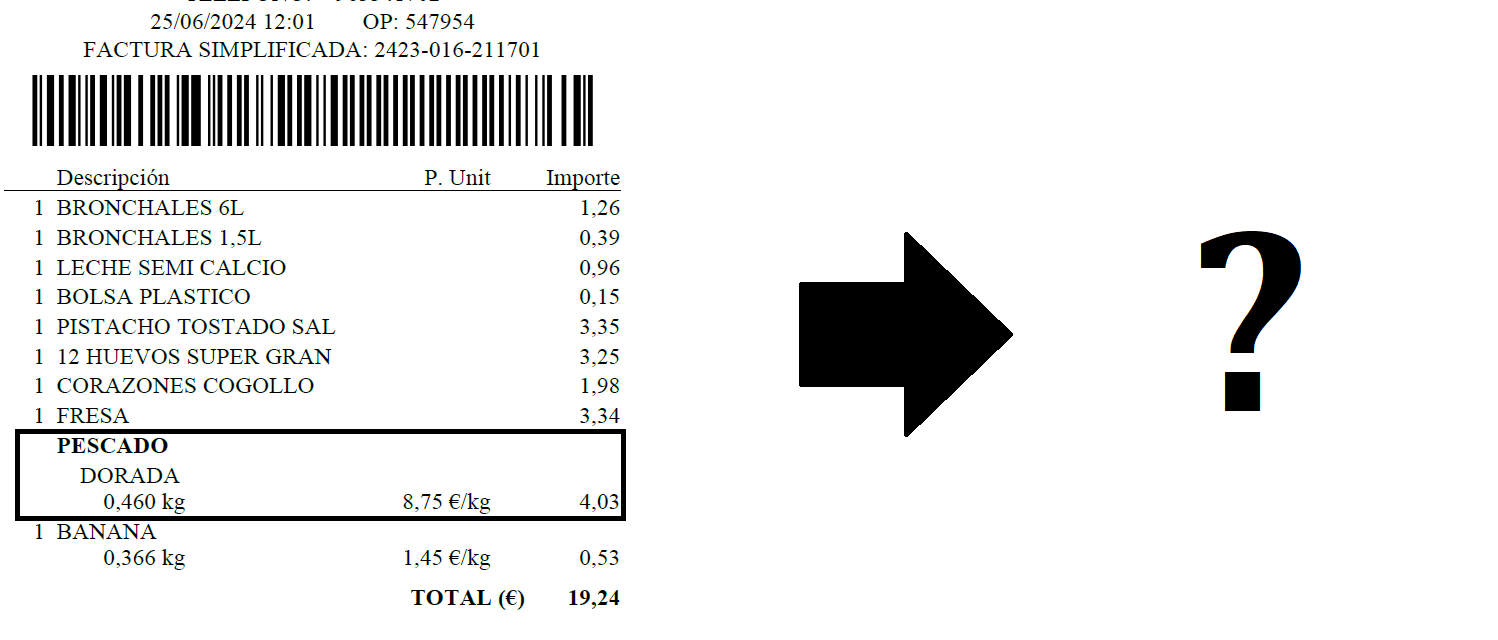
\includegraphics[width=1\linewidth]{imgEspecifiques/ticketExtraccioS}
			\caption{\textcolor{green}{Solución al conflicto}: posar solucio \textbf{TO DO TO DO}.}
			\label{fig:ticketextraccioS}
		\end{figure}
	\end{frame}
	
	
	
	
		\subsection{Front-end: Vanilla JS}
		
		\begin{frame}
			\frametitle{POSAR FRONTEND AQUI}
			
			
		\end{frame}
	
	
	
	
	
	
	
	
	
	
	
	
	
	
	
	
	
	
	
	
	
	
	
	
	
	
	
	% Sección 4
	\section{Conclusiones}
	
	\begin{frame}
		\frametitle{Conclusiones}
		\begin{itemize}
			\item Se ha aprendido a manejar tokens JWT
			\item etc etc
		\end{itemize}
	\end{frame}
	
	% Agradecimientos
	\begin{frame}
		\frametitle{Gracias por vuestra atención}
		¿Preguntas?
	\end{frame}
	
	
	
	
	
	
	
	
	

\end{document}
